%%
%% Automatically generated file from DocOnce source
%% (https://github.com/hplgit/doconce/)
%%

% #define PREAMBLE

% #ifdef PREAMBLE
%-------------------- begin preamble ----------------------

\documentclass[%
oneside,                 % oneside: electronic viewing, twoside: printing
final,                   % draft: marks overfull hboxes, figures with paths
10pt]{article}

\listfiles               % print all files needed to compile this document

\usepackage{relsize,makeidx,color,setspace,amsmath,amsfonts,amssymb}
\usepackage[table]{xcolor}
\usepackage{bm,microtype}

\usepackage[pdftex]{graphicx}

% Packages for typesetting blocks of computer code
\usepackage{fancyvrb,framed,moreverb}

% Define colors
\definecolor{orange}{cmyk}{0,0.4,0.8,0.2}
\definecolor{tucorange}{rgb}{1.0,0.64,0}
\definecolor{darkorange}{rgb}{.71,0.21,0.01}
\definecolor{darkgreen}{rgb}{.12,.54,.11}
\definecolor{myteal}{rgb}{.26, .44, .56}
\definecolor{gray}{gray}{0.45}
\definecolor{mediumgray}{gray}{.8}
\definecolor{lightgray}{gray}{.95}
\definecolor{brown}{rgb}{0.54,0.27,0.07}
\definecolor{purple}{rgb}{0.5,0.0,0.5}
\definecolor{darkgray}{gray}{0.25}
\definecolor{darkblue}{rgb}{0,0.08,0.45}
\definecolor{darkblue2}{rgb}{0,0,0.8}
\definecolor{lightred}{rgb}{1.0,0.39,0.28}
\definecolor{lightgreen}{rgb}{0.48,0.99,0.0}
\definecolor{lightblue}{rgb}{0.53,0.81,0.92}
\definecolor{lightblue2}{rgb}{0.3,0.3,1.0}
\definecolor{lightpurple}{rgb}{0.87,0.63,0.87}
\definecolor{lightcyan}{rgb}{0.5,1.0,0.83}

\colorlet{comment_green}{green!50!black}
\colorlet{string_red}{red!60!black}
\colorlet{keyword_pink}{magenta!70!black}
\colorlet{indendifier_green}{green!70!white}

% Backgrounds for code
\definecolor{cbg_gray}{rgb}{.95, .95, .95}
\definecolor{bar_gray}{rgb}{.92, .92, .92}

\definecolor{cbg_yellowgray}{rgb}{.95, .95, .85}
\definecolor{bar_yellowgray}{rgb}{.95, .95, .65}

\colorlet{cbg_yellow2}{yellow!10}
\colorlet{bar_yellow2}{yellow!20}

\definecolor{cbg_yellow1}{rgb}{.98, .98, 0.8}
\definecolor{bar_yellow1}{rgb}{.98, .98, 0.4}

\definecolor{cbg_red1}{rgb}{1, 0.85, 0.85}
\definecolor{bar_red1}{rgb}{1, 0.75, 0.85}

\definecolor{cbg_blue1}{rgb}{0.87843, 0.95686, 1.0}
\definecolor{bar_blue1}{rgb}{0.7,     0.95686, 1}

%\setlength{\fboxsep}{-1.5mm}  % adjust cod_vpad/pro_vpad background box

%% Background for code blocks (parameter is color name)

%% pro/cod_vpad: gives some vertical padding before and after the text
%% (but has more simplistic code than _cod/pro_tight+cod/pro).
%% pro/cod_vpad can be used to enclose Verbatim or lst begin/end for code.
%% pro/cod calls _pro/cod_tight and has very little vertical padding,
%% used to enclose Verbatim and other begin/end for code.
%% (pro/cod is what the ptex2tex program could produce with the
%% Blue/BlueBar definitions in .ptex2tex.cfg.)

\newenvironment{cod_vpad}[1]{
   \def\FrameCommand{\colorbox{#1}}
   \MakeFramed{\FrameRestore}}
   {\endMakeFramed}

\newenvironment{_cod_tight}[1]{
   \def\FrameCommand{\colorbox{#1}}
   \FrameRule0.6pt\MakeFramed {\FrameRestore}\vskip3mm}
   {\vskip0mm\endMakeFramed}

\newenvironment{cod}[1]{
\bgroup\rmfamily
\fboxsep=0mm\relax
\begin{_cod_tight}{#1}
\list{}{\parsep=-2mm\parskip=0mm\topsep=0pt\leftmargin=2mm
\rightmargin=2\leftmargin\leftmargin=4pt\relax}
\item\relax}
{\endlist\end{_cod_tight}\egroup}

%% Background for complete program blocks (parameter 1 is color name
%% for background, parameter 2 is color for left bar)
\newenvironment{pro_vpad}[2]{
   \def\FrameCommand{\color{#2}\vrule width 1mm\normalcolor\colorbox{#1}}
   \MakeFramed{\FrameRestore}}
   {\endMakeFramed}

\newenvironment{_pro_tight}[2]{
   \def\FrameCommand{\color{#2}\vrule width 1mm\normalcolor\colorbox{#1}}
   \FrameRule0.6pt\MakeFramed {\advance\hsize-2mm\FrameRestore}\vskip3mm}
   {\vskip0mm\endMakeFramed}

\newenvironment{pro}[2]{
\bgroup\rmfamily
\fboxsep=0mm\relax
\begin{_pro_tight}{#1}{#2}
\list{}{\parsep=-2mm\parskip=0mm\topsep=0pt\leftmargin=2mm
\rightmargin=2\leftmargin\leftmargin=4pt\relax}
\item\relax}
{\endlist\end{_pro_tight}\egroup}


\usepackage[T1]{fontenc}
%\usepackage[latin1]{inputenc}
\usepackage{ucs}
\usepackage[utf8x]{inputenc}

\usepackage{lmodern}         % Latin Modern fonts derived from Computer Modern

% Hyperlinks in PDF:
\definecolor{linkcolor}{rgb}{0,0,0.4}
\usepackage{hyperref}
\hypersetup{
    breaklinks=true,
    colorlinks=true,
    linkcolor=linkcolor,
    urlcolor=linkcolor,
    citecolor=black,
    filecolor=black,
    %filecolor=blue,
    pdfmenubar=true,
    pdftoolbar=true,
    bookmarksdepth=3   % Uncomment (and tweak) for PDF bookmarks with more levels than the TOC
    }
%\hyperbaseurl{}   % hyperlinks are relative to this root

\setcounter{tocdepth}{2}  % number chapter, section, subsection

% Tricks for having figures close to where they are defined:
% 1. define less restrictive rules for where to put figures
\setcounter{topnumber}{2}
\setcounter{bottomnumber}{2}
\setcounter{totalnumber}{4}
\renewcommand{\topfraction}{0.95}
\renewcommand{\bottomfraction}{0.95}
\renewcommand{\textfraction}{0}
\renewcommand{\floatpagefraction}{0.75}
% floatpagefraction must always be less than topfraction!
% 2. ensure all figures are flushed before next section
\usepackage[section]{placeins}
% 3. enable begin{figure}[H] (often leads to ugly pagebreaks)
%\usepackage{float}\restylefloat{figure}

\usepackage[framemethod=TikZ]{mdframed}

% --- begin definitions of admonition environments ---

% Admonition style "mdfbox" is an oval colored box based on mdframed
% "notice" admon
\colorlet{mdfbox_notice_background}{gray!5}
\newmdenv[
  skipabove=15pt,
  skipbelow=15pt,
  outerlinewidth=0,
  backgroundcolor=mdfbox_notice_background,
  linecolor=black,
  linewidth=2pt,       % frame thickness
  frametitlebackgroundcolor=blue!5,
  frametitlerule=true,
  frametitlefont=\normalfont\bfseries,
  shadow=false,        % frame shadow?
  shadowsize=11pt,
  leftmargin=0,
  rightmargin=0,
  roundcorner=5,
  needspace=0pt,
]{notice_mdfboxmdframed}

\newenvironment{notice_mdfboxadmon}[1][]{
\begin{notice_mdfboxmdframed}[frametitle=#1]
}
{
\end{notice_mdfboxmdframed}
}

% Admonition style "mdfbox" is an oval colored box based on mdframed
% "summary" admon
\colorlet{mdfbox_summary_background}{gray!5}
\newmdenv[
  skipabove=15pt,
  skipbelow=15pt,
  outerlinewidth=0,
  backgroundcolor=mdfbox_summary_background,
  linecolor=black,
  linewidth=2pt,       % frame thickness
  frametitlebackgroundcolor=blue!5,
  frametitlerule=true,
  frametitlefont=\normalfont\bfseries,
  shadow=false,        % frame shadow?
  shadowsize=11pt,
  leftmargin=0,
  rightmargin=0,
  roundcorner=5,
  needspace=0pt,
]{summary_mdfboxmdframed}

\newenvironment{summary_mdfboxadmon}[1][]{
\begin{summary_mdfboxmdframed}[frametitle=#1]
}
{
\end{summary_mdfboxmdframed}
}

% Admonition style "mdfbox" is an oval colored box based on mdframed
% "warning" admon
\colorlet{mdfbox_warning_background}{gray!5}
\newmdenv[
  skipabove=15pt,
  skipbelow=15pt,
  outerlinewidth=0,
  backgroundcolor=mdfbox_warning_background,
  linecolor=black,
  linewidth=2pt,       % frame thickness
  frametitlebackgroundcolor=blue!5,
  frametitlerule=true,
  frametitlefont=\normalfont\bfseries,
  shadow=false,        % frame shadow?
  shadowsize=11pt,
  leftmargin=0,
  rightmargin=0,
  roundcorner=5,
  needspace=0pt,
]{warning_mdfboxmdframed}

\newenvironment{warning_mdfboxadmon}[1][]{
\begin{warning_mdfboxmdframed}[frametitle=#1]
}
{
\end{warning_mdfboxmdframed}
}

% Admonition style "mdfbox" is an oval colored box based on mdframed
% "question" admon
\colorlet{mdfbox_question_background}{gray!5}
\newmdenv[
  skipabove=15pt,
  skipbelow=15pt,
  outerlinewidth=0,
  backgroundcolor=mdfbox_question_background,
  linecolor=black,
  linewidth=2pt,       % frame thickness
  frametitlebackgroundcolor=blue!5,
  frametitlerule=true,
  frametitlefont=\normalfont\bfseries,
  shadow=false,        % frame shadow?
  shadowsize=11pt,
  leftmargin=0,
  rightmargin=0,
  roundcorner=5,
  needspace=0pt,
]{question_mdfboxmdframed}

\newenvironment{question_mdfboxadmon}[1][]{
\begin{question_mdfboxmdframed}[frametitle=#1]
}
{
\end{question_mdfboxmdframed}
}

% Admonition style "mdfbox" is an oval colored box based on mdframed
% "block" admon
\colorlet{mdfbox_block_background}{gray!5}
\newmdenv[
  skipabove=15pt,
  skipbelow=15pt,
  outerlinewidth=0,
  backgroundcolor=mdfbox_block_background,
  linecolor=black,
  linewidth=2pt,       % frame thickness
  frametitlebackgroundcolor=blue!5,
  frametitlerule=true,
  frametitlefont=\normalfont\bfseries,
  shadow=false,        % frame shadow?
  shadowsize=11pt,
  leftmargin=0,
  rightmargin=0,
  roundcorner=5,
  needspace=0pt,
]{block_mdfboxmdframed}

\newenvironment{block_mdfboxadmon}[1][]{
\begin{block_mdfboxmdframed}[frametitle=#1]
}
{
\end{block_mdfboxmdframed}
}

% --- end of definitions of admonition environments ---

% prevent orhpans and widows
\clubpenalty = 10000
\widowpenalty = 10000

\newenvironment{doconceexercise}{}{}
\newcounter{doconceexercisecounter}
% --- begin definition of \listofexercises command ---
\makeatletter
\newcommand\listofexercises{\section*{List of Exercises and Problems}
\@starttoc{loe}
}
\newcommand*{\l@doconceexercise}{\@dottedtocline{0}{0pt}{6.5em}}
\makeatother
% --- end definition of \listofexercises command ---



% ------ header in subexercises ------
%\newcommand{\subex}[1]{\paragraph{#1}}
%\newcommand{\subex}[1]{\par\vspace{1.7mm}\noindent{\bf #1}\ \ }
\makeatletter
% 1.5ex is the spacing above the header, 0.5em the spacing after subex title
\newcommand\subex{\@startsection{paragraph}{4}{\z@}%
                  {1.5ex\@plus1ex \@minus.2ex}%
                  {-0.5em}%
                  {\normalfont\normalsize\bfseries}}
\makeatother


% --- end of standard preamble for documents ---


% insert custom LaTeX commands...

\raggedbottom
\makeindex
\usepackage[totoc]{idxlayout}   % for index in the toc
\usepackage[nottoc]{tocbibind}  % for references/bibliography in the toc

%-------------------- end preamble ----------------------

\begin{document}

% matching end for #ifdef PREAMBLE
% #endif

\newcommand{\half}{\frac{1}{2}}
\newcommand{\halfi}{{1/2}}
\newcommand{\tp}{\thinspace .}

\newcommand{\uex}{{u_{\small\mbox{e}}}}
\newcommand{\uexd}[1]{{u_{\small\mbox{e}, #1}}}
\newcommand{\vex}{{v_{\small\mbox{e}}}}
\newcommand{\vexd}[1]{{v_{\small\mbox{e}, #1}}}
\newcommand{\Aex}{{A_{\small\mbox{e}}}}

% Operators
\newcommand{\Ddt}[1]{\frac{D #1}{dt}}
\newcommand{\E}[1]{\hbox{E}\lbrack #1 \rbrack}
\newcommand{\Var}[1]{\hbox{Var}\lbrack #1 \rbrack}
\newcommand{\Std}[1]{\hbox{Std}\lbrack #1 \rbrack}

\newcommand{\xpoint}{\bm{x}}
\newcommand{\normalvec}{\bm{n}}
\newcommand{\Oof}[1]{\mathcal{O}(#1)}

% Boldface vectors/tensors
\newcommand{\x}{\bm{x}}
\newcommand{\X}{\bm{X}}
\renewcommand{\u}{\bm{u}}
\renewcommand{\v}{\bm{v}}
\newcommand{\w}{\bm{w}}
\newcommand{\acc}{\bm{a}}
\newcommand{\rpos}{\bm{r}}
\newcommand{\V}{\bm{V}}
\newcommand{\e}{\bm{e}}
\newcommand{\f}{\bm{f}}
\newcommand{\F}{\bm{F}}
\newcommand{\stress}{\bm{\sigma}}
\newcommand{\strain}{\bm{\varepsilon}}
\newcommand{\stressc}{{\sigma}}
\newcommand{\strainc}{{\varepsilon}}
\newcommand{\I}{\bm{I}}
\newcommand{\T}{\bm{T}}

\newcommand{\dfc}{\alpha}  % diffusion coefficient
% Unit vectors
\newcommand{\ii}{\bm{i}}
\newcommand{\jj}{\bm{j}}
\newcommand{\kk}{\bm{k}}
\newcommand{\ir}{\bm{i}_r}
\newcommand{\ith}{\bm{i}_{\theta}}
\newcommand{\iz}{\bm{i}_z}

% Index sets
\newcommand{\Ix}{\mathcal{I}_x}
\newcommand{\Iy}{\mathcal{I}_y}
\newcommand{\Iz}{\mathcal{I}_z}
\newcommand{\It}{\mathcal{I}_t}
%\newcommand{\Ix}{{I_x}}
%\newcommand{\Iy}{{I_y}}
%\newcommand{\Iz}{{I_z}}
%\newcommand{\It}{{I_t}}
%\newcommand{\If}{\mathcal{I}}     % for FEM
\newcommand{\If}{\mathcal{I}_s}     % for FEM
%\newcommand{\If}{{I}}     % for FEM
%\newcommand{\Ifd}{\mathcal{I}_d}  % for FEM
\newcommand{\Ifd}{{I_d}}  % for FEM
\newcommand{\Ifb}{{I_b}}  % for FEM
\newcommand{\setb}[1]{#1^0}    % set begin
\newcommand{\sete}[1]{#1^{-1}} % set end
%\newcommand{\setl}[1]{#1\setminus\{\set1{#1}\}}
%\newcommand{\setr}[1]{#1\setminus\{\set0{#1}\}}
%\newcommand{\seti}[1]{#1\setminus\{\set0{#1},\set1{#1}\}}
\newcommand{\setl}[1]{#1^-}
\newcommand{\setr}[1]{#1^+}
\newcommand{\seti}[1]{#1^i}
\newcommand{\sequencei}[1]{\left\{ {#1}_i \right\}_{i\in\If}}

% Finite elements
\newcommand{\basphi}{\varphi}
\newcommand{\baspsi}{\psi}
\newcommand{\refphi}{\tilde\basphi}
\newcommand{\psib}{\bm{\psi}}
\newcommand{\sinL}[1]{\sin\left((#1+1)\pi\frac{x}{L}\right)}
\newcommand{\xno}[1]{x_{#1}}
%\newcommand{\xno}[1]{x^{(#1)}}
\newcommand{\Xno}[1]{X_{(#1)}}
\newcommand{\yno}[1]{y_{#1}}
\newcommand{\Yno}[1]{Y_{(#1)}}
\newcommand{\xdno}[1]{\bm{x}_{#1}}

% FEniCS commands
\newcommand{\dX}{\, \mathrm{d}X}
\newcommand{\dx}{\, \mathrm{d}x}
\newcommand{\ds}{\, \mathrm{d}s}
\newcommand{\Real}{\mathbb{R}}
\newcommand{\Integerp}{\mathbb{N}}
\newcommand{\Integer}{\mathbb{Z}}


% ------------------- main content ----------------------



% ----------------- title -------------------------

\thispagestyle{empty}

\begin{center}
{\LARGE\bf
\begin{spacing}{1.25}
Algorithms and implementations for exponential decay models
\end{spacing}
}
\end{center}

% ----------------- author(s) -------------------------

\begin{center}
{\bf Hans Petter Langtangen${}^{1, 2}$} \\ [0mm]
\end{center}

\begin{center}
% List of all institutions:
\centerline{{\small ${}^1$Center for Biomedical Computing, Simula Research Laboratory}}
\centerline{{\small ${}^2$Department of Informatics, University of Oslo}}
\end{center}
    
% ----------------- end author(s) -------------------------

% --- begin date ---
\begin{center}
Oct 18, 2015
\end{center}
% --- end date ---

\vspace{1cm}


\tableofcontents

\clearpage % pagebreak before list of exercises
\subsection*{List of Exercises and Problems}
\begin{tabular}{lrll}
Exercise & 1 & Define a mesh function and visualize it & p.~\pageref{decay:exer:meshfunc} \\
Problem & 2 & Differentiate a function & p.~\pageref{decay:exer:dudt} \\
Problem & 3 & Experiment with divisions & p.~\pageref{decay:exer:intdiv} \\
Problem & 4 & Experiment with wrong computations & p.~\pageref{decay:exer:decay1err} \\
Problem & 5 & Plot the error function & p.~\pageref{decay:exer:plot:error} \\
Problem & 6 & Change formatting of numbers and debug & p.~\pageref{decay:exer:inexact:output} \\
\end{tabular}
% --- end of table of exercises
\clearpage % pagebreak after list of exercises




\vspace{1cm} % after toc








% !split
Throughout industry and science it is common today to study nature or
technological devices through models on a computer. With such models
the computer acts as a virtual lab where experiments can be done
in a fast, reliable, safe, and cheap way. In some fields, e.g., aerospace
engineering, the computer models are now so sophisticated that they
can replace physical experiments to a large extent.

% Computational science is a widely used term for doing scientific discoveries
% using computer models. Similarly, computational engineering is about
% engineering based on heavy use of computer models. The present book does
% not cover how to do scientific discoveries or engineering, but
% targets how to create reliable computer models. This task is often
% called scientific computing

A vast amount of computer models are based on ordinary and partial
differential equations. This book is an introduction to the
various scientific ingredients we need for reliable computing with such
type of models. A key theme is to solve differential equations
\emph{numerically} on a computer. Many methods are available for this purpose,
but the focus here is on \emph{finite difference methods}, because these
are simple, yet versatile, for solving a wide range of ordinary and
partial differential equations. The present chapter first presents the
mathematical ideas of finite difference methods and derives algorithms,
i.e., formulations of the methods ready for computer programming.
Then we create programs and learn how we can be sure that the programs
really work correctly.


\section{Finite difference methods}

\label{decay:basics}

This section explains the basic ideas of finite difference methods
via the simple ordinary differential equation $u^{\prime}=-au$.
Emphasis is put on the reasoning behind problem discretizing and
introduction of key concepts such as mesh, mesh function,
finite difference approximations, averaging in a mesh,
derivation of algorithms, and discrete operator notation.


\subsection{A basic model for exponential decay}
\label{decay:model}

\index{decay ODE} \index{exponential decay}

Our model problem is perhaps the simplest ordinary differential
equation (ODE):

\begin{equation*}
u^{\prime}(t) = -au(t)\tp
\end{equation*}
In this equation, $u(t)$ is a scalar function of time $t$,
$a$ is a constant (in this book we mostly work with $a>0$),
and $u^{\prime}(t)$ means differentiation with
respect to $t$. This type of equation arises in a number of
widely different phenomena where some quantity $u$ undergoes
exponential reduction (provided $a>0$).
Examples include radioactive decay, population
decay, investment decay, cooling of an object, pressure decay in the
atmosphere, and retarded motion in fluids. Some models with growth,
$a<0$, are treated as
well.
We have chosen this particular ODE not only because
its applications are relevant, but even more because studying
numerical solution methods for this particular ODE gives important insight
that can be reused in far more complicated settings, in particular
when solving diffusion-type partial differential equations.

\paragraph{The exact solution.}
Although our interest is in \emph{approximate} numerical solutions of
$u^{\prime}=-au$, it is convenient to know the exact analytical
solution of the problem so we can compute the error in numerical
approximations.  The analytical solution of this ODE is found by
separation of variables, which results in

\begin{equation*} u(t) = Ce^{-at},\end{equation*}
for any arbitrary constant $C$.
To obtain a unique solution, we need a condition to fix the value of $C$.
This condition is known as the \emph{initial condition} and stated as
$u(0)=I$. That is, we know that the value of $u$ is $I$ when the process
starts at $t=0$. With this knowledge, the exact solution becomes
$u(t)=Ie^{-at}$. The initial condition is also crucial for numerical
methods: without it, we can never start the numerical algorithms!

\paragraph{A complete problem formulation.}
Besides an initial condition for the ODE, we also need to specify a
time interval for the solution: $t\in (0,T]$.
The point $t=0$ is not
included since we know that $u(0)=I$ and assume that the equation governs
$u$ for $t>0$.
Let us now summarize the information that is required to
state the complete problem formulation:
find $u(t)$
such that

\begin{equation}
u^{\prime} = -au,\ t\in (0,T], \quad u(0)=I\tp   \label{decay:problem}
\end{equation}
This is known as a \emph{continuous problem} because the parameter $t$
varies continuously from $0$ to $T$. For each $t$ we have a corresponding
$u(t)$. There are hence infinitely many values of $t$ and $u(t)$.
The purpose of a numerical method is to formulate a corresponding
\emph{discrete} problem whose solution is characterized by a finite number of values,
which can be computed in a finite number of steps on a computer.
Typically, we choose a finite set of time values $t_0,t_1,\ldots,t_{N_t}$,
and create algorithms that generate the corresponding $u$ values
$u_0,u_1,\ldots,u_{N_t}$.


\subsection{The Forward Euler scheme}
\label{decay:schemes:FE}

Solving an ODE like (\ref{decay:problem}) by a finite difference method
consists of the following four steps:

\begin{enumerate}
\item discretizing the domain,

\item requiring fulfillment of the equation at discrete time points,

\item replacing derivatives by finite differences,

\item formulating a recursive algorithm.
\end{enumerate}

\noindent
\index{mesh} \index{grid}

\paragraph{Step 1: Discretizing the domain.}
The time domain $[0,T]$ is represented by a finite number of
$N_t+1$ points

\begin{equation}
0 = t_0 < t_1 < t_2 < \cdots < t_{N_t-1} < t_{N_t} = T\tp
\end{equation}
The collection of points $t_0,t_1,\ldots,t_{N_t}$ constitutes a \emph{mesh}
or \emph{grid}. Often the mesh points will be uniformly spaced in
the domain $[0,T]$, which means that the spacing $t_{n+1}-t_n$ is
the same for all $n$. This spacing is often denoted by $\Delta t$,
which means that $t_n=n\Delta t$.

\index{mesh function}

We want the solution $u$ at the mesh points:
$u(t_n)$, $n=0,1,\ldots,N_t$.
A notational short-form for $u(t_n)$,
which will be used extensively, is $u^{n}$. More precisely, we let
$u^n$ be the \emph{numerical approximation} to the exact solution $u(t_n)$
at $t=t_n$.

When we need to clearly distinguish between the numerical and exact solution,
we often place a subscript e on the exact solution, as in $\uex(t_n)$.
Figure~\ref{decay:fdu:e} shows the $t_n$ and $u^n$ points for $n=0,1,\ldots,N_t=7$ as well as $\uex(t)$ as the dashed line.


\begin{figure}[!ht]  % decay:fdu:e
  \centerline{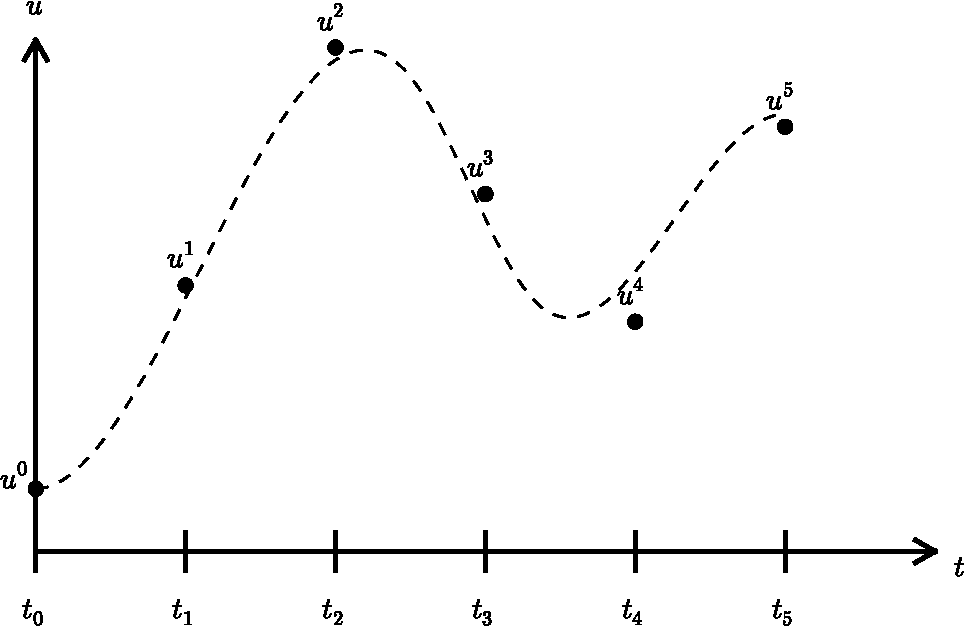
\includegraphics[width=1.0\linewidth]{fig-alg/fdm_u_ue.pdf}}
  \caption{
  Time mesh with discrete solution values at points and a dashed line indicating the true solution. \label{decay:fdu:e}
  }
\end{figure}
%\clearpage % flush figures decay:fdu:e



We say that the numerical approximation, i.e.,
the collection of $u^n$ values for $n=0,\ldots,N_t$,
constitutes a \emph{mesh function}.
A ``normal'' continuous function is a curve defined for all real $t$
values in $[0,T]$, but a mesh function is only defined at discrete
points in time. If you want to compute the mesh function \emph{between} the
mesh points, where it is not defined, an \emph{interpolation method} must be
used. Usually, linear interpolation, i.e., drawing a straight line between
the mesh function values, see Figure~\ref{decay:fdu:e}, suffices.
To compute the solution for some $t\in [t_n, t_{n+1}]$, we use the
linear interpolation formula

\begin{equation}
u(t) \approx u^n + \frac{u^{n+1}-u^n}{t_{n+1}-t_n}(t - t_n)\tp
\end{equation}


\begin{figure}[!ht]  % decay:fdu:ei
  \centerline{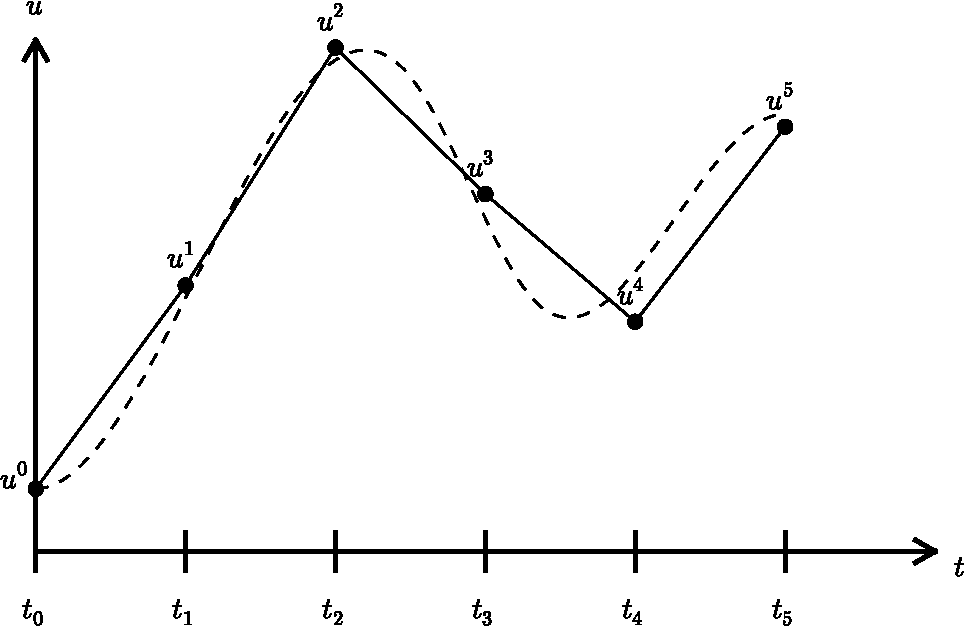
\includegraphics[width=1.0\linewidth]{fig-alg/fdm_u_uei.pdf}}
  \caption{
  Linear interpolation between the discrete solution values (dashed curve is exact solution). \label{decay:fdu:ei}
  }
\end{figure}
%\clearpage % flush figures decay:fdu:ei


\clearpage


\begin{notice_mdfboxadmon}[Notice.]
The goal of a numerical solution method for ODEs is
to compute the mesh function by solving a finite set of
\emph{algebraic equations} derived from the original ODE problem.
\end{notice_mdfboxadmon}



\paragraph{Step 2: Fulfilling the equation at discrete time points.}
The ODE is supposed to hold for all $t\in (0,T]$, i.e., at an infinite
number of points. Now we relax that requirement and require that
the ODE is fulfilled at a finite set of discrete points in time.
The mesh points $t_0,t_1,\ldots,t_{N_t}$ are a natural
(but not the only) choice of points.
The original ODE is then reduced to  the following equations:

\begin{equation}
u^{\prime}(t_n) = -au(t_n),\quad n=0,\ldots,N_t,\quad u(0)=I\tp
\label{decay:step2}
\end{equation}
Even though the original ODE is not stated to be valid at $t=0$, it
is valid as close to $t=0$ as we like, and it turns out that it
is useful for construction of numerical methods to have
(\ref{decay:step2}) valid for $n=0$. The next two steps show that we
need (\ref{decay:step2}) for $n=0$.

\index{finite differences}

\paragraph{Step 3: Replacing derivatives by finite differences.}
The next and most essential step of the method is to replace the
derivative $u^{\prime}$ by a finite difference approximation. Let us first
try a \emph{forward} difference approximation (see Figure~\ref{decay:sketch:FE}),

\index{forward difference} \index{finite differences!forward}

\begin{equation}
u^{\prime}(t_n) \approx \frac{u^{n+1}-u^{n}}{t_{n+1}-t_n}\tp
\label{decay:FEdiff}
\end{equation}
The name forward relates to the fact that we use a value forward in
time, $u^{n+1}$, together with the value $u^n$ at the point $t_n$, where
we seek the derivative, to approximate $u^{\prime}(t_n)$.
Inserting this approximation in (\ref{decay:step2}) results in

\begin{equation}
\frac{u^{n+1}-u^{n}}{t_{n+1}-t_n} = -au^{n},\quad n=0,1,\ldots,N_t-1\tp
\label{decay:step3}
\end{equation}
Note that if we want to compute the solution
up to time level $N_t$,
we only need (\ref{decay:step2}) to hold for $n=0,\ldots,N_t-1$ since
(\ref{decay:step3}) for $n=N_t-1$ creates an equation for the final
value $u^{N_t}$.

Also note that we use the approximation symbol $\approx$ in (\ref{decay:FEdiff}),
but not in (\ref{decay:step3}). Instead, we view (\ref{decay:step3}) as
an equation that is not mathematically equivalent to (\ref{decay:FEdiff}),
but represents an approximation to the equation (\ref{decay:FEdiff}).

Equation (\ref{decay:step3})
is the discrete counterpart to the original ODE problem
(\ref{decay:problem}), and often referred to as a \emph{finite difference scheme}
or more generally as the \emph{discrete equations} of the problem.
The fundamental feature of these equations is that they are \emph{algebraic}
and can hence be straightforwardly solved to produce the mesh function, i.e.,
the approximate values of $u$ at
the mesh points: $u^n$, $n=1,2,\ldots,N_t$.


\begin{figure}[!ht]  % decay:sketch:FE
  \centerline{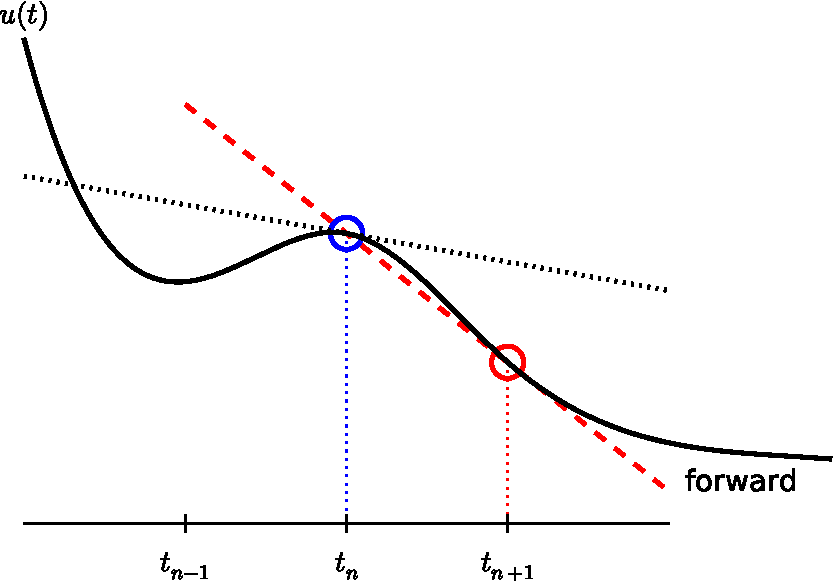
\includegraphics[width=0.8\linewidth]{fig-alg/fd_forward.pdf}}
  \caption{
  Illustration of a forward difference. \label{decay:sketch:FE}
  }
\end{figure}
%\clearpage % flush figures decay:sketch:FE


\index{difference equation}
\index{discrete equation}
\index{algebraic equation}
\index{finite difference scheme}
\index{Forward Euler scheme}

\paragraph{Step 4: Formulating a recursive algorithm.}
The final step is to identify the computational algorithm to be implemented
in a program. The key observation here is to realize that
(\ref{decay:step3}) can be used to compute $u^{n+1}$ if $u^n$ is known.
Starting with $n=0$, $u^0$ is known since $u^0=u(0)=I$, and
(\ref{decay:step3}) gives an equation for $u^1$. Knowing $u^1$,
$u^2$ can be found from (\ref{decay:step3}). In general, $u^n$
in (\ref{decay:step3}) can be assumed known, and then we can easily solve for
the unknown $u^{n+1}$:

\begin{equation}
u^{n+1} = u^n - a(t_{n+1} -t_n)u^n\tp
\label{decay:FE}
\end{equation}
We shall refer to (\ref{decay:FE}) as the Forward Euler (FE) scheme
for our model problem. From a mathematical point of view,
equations of the form (\ref{decay:FE}) are known as
\emph{difference equations} since they express how differences in
the dependent variable, here $u$, evolve with $n$. In our case,
the differences in $u$ are given by $u^{n+1}-u^n = -a(t_{n+1}-t_n)u^n$.
The finite difference method can be viewed as a method for turning
a differential equation into an algebraic difference equation that
can be easily solved by repeated use of a formula like (\ref{decay:FE}).

\paragraph{Interpretation.}
There is a very intuitive interpretation of the FE scheme, illustrated
in the sketch below. We have computed some point values
on the solution curve (small red disks), and the question is how we reason
about the next point. Since we know $u$ and $t$ at the most recently
computed point, the differential equation gives us the \emph{slope} of
the solution curve: $u'=-au$. We can draw this slope as a red line
and continue the solution curve along that slope. As soon as we have
chosen the next point on this line, we have a new $t$ and $u$ value and
can compute a new slope and continue the process.



\vspace{3mm}




\vspace{3mm}





% inline figure
\centerline{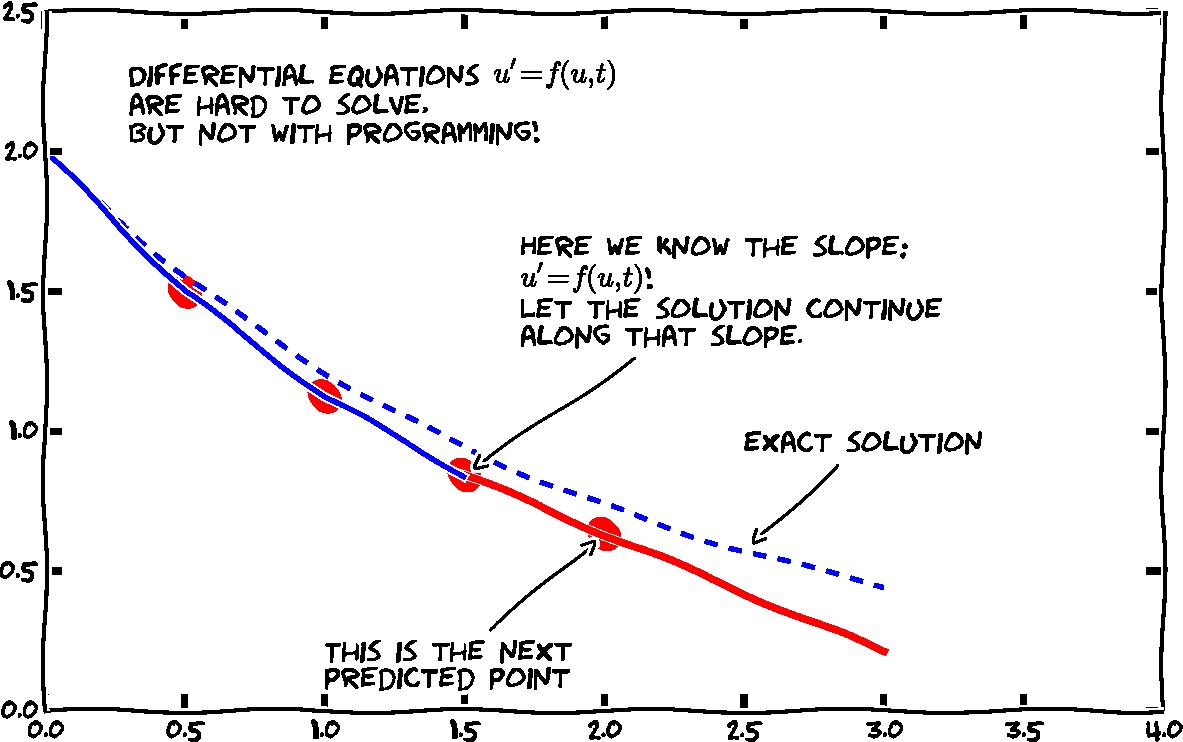
\includegraphics[width=0.8\linewidth]{fig-alg/FE_idea.pdf}}





\vspace{3mm}




\vspace{3mm}



\paragraph{Computing with the recursive formula.}
Mathematical computation with (\ref{decay:FE}) is straightforward:

\begin{align*}
u_0 &= I,\\ 
u_1 & = u^0 - a(t_{1} -t_0)u^0 = I(1-a(t_1-t_0)),\\ 
u_2 & = u^1 - a(t_{2} -t_1)u^1 = I(1-a(t_1-t_0))(1 - a(t_2-t_1)),\\ 
u^3 &= u^2 - a(t_{3} -t_2)u^2 = I(1-a(t_1-t_0))(1 - a(t_2-t_1))(1 - a(t_3-t_2)),
\end{align*}
and so on until we reach $u^{N_t}$.
Very often, $t_{n+1}-t_n$ is constant for all $n$, so we can introduce
the common symbol
$\Delta t = t_{n+1}-t_n$, $n=0,1,\ldots,N_t-1$.
Using a constant mesh spacing $\Delta t$ in the above calculations gives

\begin{align*}
u_0 &= I,\\ 
u_1 & = I(1-a\Delta t),\\ 
u_2 & = I(1-a\Delta t)^2,\\ 
u^3 &= I(1-a\Delta t)^3,\\ 
&\vdots\\ 
u^{N_t} &= I(1-a\Delta t)^{N_t}\tp
\end{align*}
This means that we have found a closed formula for $u^n$, and there is
no need to let a computer generate the sequence $u^1, u^2, u^3, \ldots$.
However, finding such a formula for $u^n$ is possible only for a few very
simple problems, so in general finite difference equations must be
solved on a computer.

As the next sections will show, the scheme (\ref{decay:FE}) is just one
out of many alternative finite difference (and other) methods for
the model problem (\ref{decay:problem}).

\subsection{The Backward Euler scheme}
\label{decay:schemes:BE}

\index{backward difference} \index{finite differences!backward}

There are several choices of difference approximations in step 3 of
the finite difference method as presented in the previous section.
Another alternative is

\begin{equation}
u^{\prime}(t_n) \approx \frac{u^{n}-u^{n-1}}{t_{n}-t_{n-1}}\tp
\label{decay:BEdiff}
\end{equation}
Since this difference is based on going backward in time ($t_{n-1}$)
for information, it is known as a \emph{backward} difference, also called
Backward Euler difference.
Figure~\ref{decay:sketch:BE} explains the idea.


\begin{figure}[!ht]  % decay:sketch:BE
  \centerline{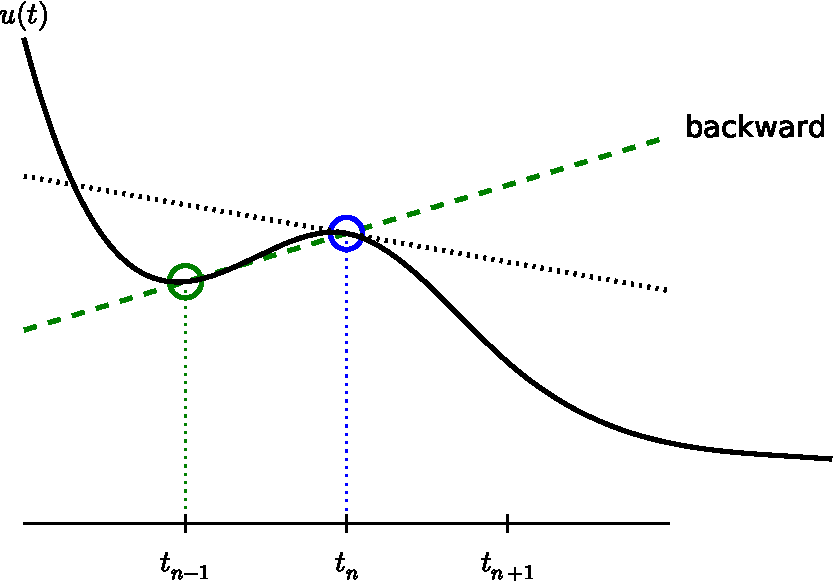
\includegraphics[width=0.8\linewidth]{fig-alg/fd_backward.pdf}}
  \caption{
  Illustration of a backward difference. \label{decay:sketch:BE}
  }
\end{figure}
%\clearpage % flush figures decay:sketch:BE


\index{backward scheme, 1-step}
\index{Backward Euler scheme}

Inserting (\ref{decay:BEdiff}) in (\ref{decay:step2}) yields
the Backward Euler (BE) scheme:

\begin{equation}
\frac{u^{n}-u^{n-1}}{t_{n}-t_{n-1}} = -a u^n,\quad n=1,\ldots,N_t\tp
\label{decay:BE0}
\end{equation}
We assume, as explained under step 4 in Section~\ref{decay:schemes:FE},
that we have computed $u^0, u^1, \ldots, u^{n-1}$ such that
(\ref{decay:BE0}) can be used to compute $u^n$. Note that
(\ref{decay:BE0}) needs $n$ to start at 1 (then it involves $u^0$, but
no $u^{-1}$) and end at $N_t$.

For direct similarity with the formula for the
Forward Euler scheme (\ref{decay:FE})
we replace $n$ by $n+1$ in (\ref{decay:BE0}) and solve for the
unknown value $u^{n+1}$:

\begin{equation}
u^{n+1} = \frac{1}{1+ a(t_{n+1}-t_n)} u^n,\quad n=0,\ldots,N_t-1\tp
\label{decay:BE}
\end{equation}

\subsection{The Crank-Nicolson scheme}
\label{decay:schemes:CN}

\index{Crank-Nicolson scheme}
\index{centered difference} \index{finite differences!centered}


The finite difference approximations
(\ref{decay:FEdiff}) and (\ref{decay:BEdiff}) used to derive the schemes
(\ref{decay:FE}) and (\ref{decay:BE}), respectively,
are both one-sided differences, i.e.,
we collect information either forward or backward in time when approximating
the derivative at a point. Such one-sided differences are
known to be less accurate than central (or midpoint)
differences, where we use information both forward and backward in
time. A natural next step is therefore to construct
a central difference approximation that will yield a more accurate
numerical solution.

The central difference approximation to the derivative is sought at the
point $t_{n+\half}=\half (t_n + t_{n+1})$ (or
$t_{n+\half}=(n+\half)\Delta t$ if the mesh spacing is uniform in time).
The approximation reads

\begin{equation}
u^{\prime}(t_{n+\half}) \approx \frac{u^{n+1}-u^n}{t_{n+1}-t_n}\tp
\label{decay:CNdiff}
\end{equation}
Figure~\ref{decay:sketch:CN} sketches the geometric interpretation of
such a centered difference.
Note that the fraction on the right-hand side is the same as for the
Forward Euler approximation (\ref{decay:FEdiff}) and
the Backward Euler approximation (\ref{decay:BEdiff}) (with
$n$ replaced by $n+1$). The accuracy of this fraction as an approximation
to the derivative of $u$ depends on \emph{where} we seek the derivative:
in the center of the interval $[t_{n},t_{n+1}]$ or at the end points.
We shall later see that it is more accurate at the center point.


\begin{figure}[!ht]  % decay:sketch:CN
  \centerline{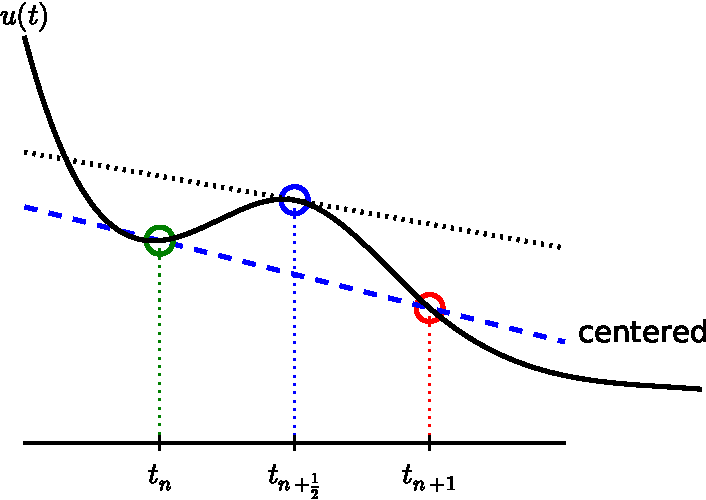
\includegraphics[width=0.8\linewidth]{fig-alg/fd_centered_CN.pdf}}
  \caption{
  Illustration of a centered difference. \label{decay:sketch:CN}
  }
\end{figure}
%\clearpage % flush figures decay:sketch:CN


With the formula (\ref{decay:CNdiff}), where $u^{\prime}$ is evaluated at
$t_{n+\half}$, it is natural to demand the
ODE to be fulfilled at the time points \emph{between} the mesh points:

\begin{equation}
u^{\prime}(t_{n+\half}) = -au(t_{n+\half}),\quad n=0,
\ldots,N_t-1\tp
\label{decay:step2m}
\end{equation}
Using (\ref{decay:CNdiff}) in (\ref{decay:step2m}) results in
the approximate discrete equation

\begin{equation}
\frac{u^{n+1}-u^n}{t_{n+1}-t_n} = -au^{n+\half},\quad n=0,\ldots,N_t-1,
\label{decay:CN0}
\end{equation}
where $u^{n+\half}$ is a short form for the numerical approximation
to $u(t_{n+\half})$.

There is a fundamental problem with the right-hand side of
(\ref{decay:CN0}): we aim to compute $u^n$ for integer $n$, which means
that $u^{n+\half}$ is not a quantity computed by our method. The
quantity must
therefore be
expressed by the quantities that we actually produce, i.e.,
the numerical solution at the
mesh points. One possibility is to approximate $u^{n+\half}$
as an arithmetic mean of the $u$ values at the neighboring mesh points:

\index{averaging!arithmetic}

\begin{equation}
u^{n+\half} \approx \half (u^n + u^{n+1})\tp
\label{decay:uhalfavg}
\end{equation}
Using (\ref{decay:uhalfavg}) in (\ref{decay:CN0}) results in a new
approximate discrete equation

\begin{equation}
\frac{u^{n+1}-u^n}{t_{n+1}-t_n} = -a\half (u^n + u^{n+1})\tp
\label{decay:CN1}
\end{equation}
There are three approximation steps leading to this formula:
1) the ODE is only valid at discrete points (between the mesh points),
2) the derivative is approximated by a finite difference, and 3) the
value of $u$ between mesh points is approximated by an arithmetic mean
value. Despite one more approximation than for the Backward and Forward
Euler schemes, the use of a centered difference leads to a more
accurate method.

To formulate a recursive algorithm,
we assume that $u^n$ is already computed so that $u^{n+1}$ is the
unknown, which we can solve for:

\begin{equation}
u^{n+1} = \frac{1-\half a(t_{n+1}-t_n)}{1 + \half a(t_{n+1}-t_n)}u^n\tp
\label{decay:CN}
\end{equation}
The finite difference scheme (\ref{decay:CN}) is often called
the Crank-Nicolson (CN) scheme or a midpoint or centered scheme.
Note that (\ref{decay:CN}) as well as (\ref{decay:FE}) and (\ref{decay:BE})
apply whether the spacing in the time mesh, $t_{n+1}-t_n$, depends on $n$
or is constant.


\subsection{The unifying $\theta$-rule}
\label{decay:schemes:theta}

\index{weighted average} \index{theta-rule} \index{$\theta$-rule}

The Forward Euler, Backward Euler, and Crank-Nicolson schemes can be
formulated as one scheme with a varying parameter $\theta$:

\begin{equation}
\frac{u^{n+1}-u^{n}}{t_{n+1}-t_n} = -a (\theta u^{n+1} + (1-\theta) u^{n})
\label{decay:th0}
\tp
\end{equation}

Observe that

\begin{itemize}
 \item $\theta =0$ gives the Forward Euler scheme

 \item $\theta =1$ gives the Backward Euler scheme,

 \item $\theta =\half$ gives the Crank-Nicolson scheme.
\end{itemize}

\noindent
One may alternatively choose any other value of $\theta$ in $[0,1]$, but
this is not so common since the accuracy and stability of
the scheme do not improve compared
to the values $\theta=0,1,\half$.

As before, $u^n$ is considered known and $u^{n+1}$ unknown, so
we solve for the latter:

\begin{equation}
u^{n+1} = \frac{1 - (1-\theta) a(t_{n+1}-t_n)}{1 + \theta a(t_{n+1}-t_n)}\tp
\label{decay:th}
\end{equation}
This scheme is known as the $\theta$-rule, or alternatively written as
the ``theta-rule''.


\begin{notice_mdfboxadmon}[Derivation.]
We start with replacing $u^{\prime}$ by the fraction

\begin{equation*} \frac{u^{n+1}-u^{n}}{t_{n+1}-t_n},\end{equation*}
in the Forward Euler, Backward Euler,
and Crank-Nicolson schemes. Then we observe that
the difference between the methods concerns which point this
fraction approximates the derivative. Or in other words, at which point we
sample the ODE. So far this has been the
end points or the midpoint of $[t_n,t_{n+1}]$. However, we may choose any point
$\tilde t \in [t_n,t_{n+1}]$.
The difficulty
is that evaluating the right-hand side $-au$ at an arbitrary point
faces the same problem as in
Section~\ref{decay:schemes:CN}: the point value must be expressed
by the discrete $u$ quantities that we compute by the scheme, i.e.,
$u^n$ and $u^{n+1}$. Following the averaging idea from
Section~\ref{decay:schemes:CN},
the value of $u$ at an arbitrary point $\tilde t$ can be
calculated as a \emph{weighted average}, which generalizes the arithmetic mean
$\half u^n + {\half}u^{n+1}$.
The weighted average reads

\begin{equation}
u(\tilde t) \approx \theta u^{n+1} + (1-\theta) u^{n},
\label{decay:thetaavg_u}
\end{equation}
where $\theta\in [0,1]$ is a weighting factor.
We can also express $\tilde t$ as a similar weighted average

\begin{equation}
\tilde t \approx \theta t_{n+1} + (1-\theta) t_{n}\tp
\label{decay:thetaavg_t}
\end{equation}

Let now the ODE hold at the point
$\tilde t\in [t_n,t_{n+1}]$, approximate $u^{\prime}$ by the fraction
$(u^{n+1}-u^{n})/(t_{n+1}-t_n)$, and approximate the right-hand
side $-au$ by the weighted average (\ref{decay:thetaavg_u}).
The result is (\ref{decay:th0}).
\end{notice_mdfboxadmon}



\subsection{Constant time step}

All schemes up to now have been formulated for a general non-uniform
mesh in time: $t_0 < t_1 < \cdots < t_{N_t}$.
Non-uniform meshes are highly relevant
since one can use many points in regions where $u$ varies rapidly, and
fewer points in regions where $u$ is slowly varying. This idea saves
the total number of points and therefore makes it faster to compute the mesh
function $u^n$. Non-uniform meshes are used together with
\emph{adaptive} methods that are able to adjust the time mesh during the
computations.

\index{time step}

However, a uniformly distributed set of mesh points is not only
convenient, but also
sufficient for many applications. Therefore, it is a very common
choice. We shall
present the finite difference schemes for a uniform point distribution
$t_n=n\Delta t$, where $\Delta t$ is the constant spacing between
the mesh points, also referred to as the \emph{time step}.
The resulting formulas look simpler and are more
well known.


\begin{summary_mdfboxadmon}[Summary of schemes for constant time step.]
\begin{alignat}{2}
u^{n+1} &= (1 - a\Delta t )u^n  & \hbox{Forward Euler}
\label{decay:FE:u}\\ 
u^{n+1} &= \frac{1}{1+ a\Delta t} u^n  & \hbox{Backward Euler}
\label{decay:BE:u}\\ 
u^{n+1} &= \frac{1-\half a\Delta t}{1 + \half a\Delta t} u^n & \hbox{Crank-Nicolson}
\label{decay:CN:u}\\ 
u^{n+1} &= \frac{1 - (1-\theta) a\Delta t}{1 + \theta a \Delta t}u^n  & \hbox{The }\theta-\hbox{rule}
\label{decay:th:u}
\end{alignat}
\end{summary_mdfboxadmon}



It is not accidental that we focus on presenting the Forward Euler, Backward
Euler, and Crank-Nicolson schemes. They complement each other with their
different pros and cons, thus providing a useful collection of
solution methods for many differential equation problems.
The unifying notation of the $\theta$-rule makes it convenient to
work with all three methods through just one formula. This is
particularly advantageous in computer implementations since one avoids
if-else tests with formulas that have repetitive elements.


\subsection{Mathematical derivation of finite difference formulas}
\label{decay:fd:taylor}

The finite difference formulas for approximating the first derivative
of a function have so far been somewhat justified through graphical
illustrations in Figures~\ref{decay:sketch:FE}, \ref{decay:sketch:BE},
and~\ref{decay:sketch:CN}. The task is to approximate the derivative
at a point of a curve using only two function values. By drawing
a straight line through the points, we have some approximation to
the tangent of the curve and use the slope of this line as
an approximation to the derivative. The slope can be computed by
inspecting the figures.

However, we can alternatively derive the finite difference formulas by
pure mathematics. The key tool for this approach is Taylor series,
or more precisely, approximation of functions by lower-order
Taylor polynomials. Given a function $f(x)$ that is sufficiently
smooth (i.e., $f(x)$ has ``enough derivatives''),
a Taylor polynomial of degree $m$ can be used to approximate the
value of the function $f(x)$ if we know the values of $f$ and its
first $m$ derivatives at some other point $x=a$. The formula for the
Taylor polynomial reads

\begin{align}
f(x) & \approx f(a) + f'(a)(x-a) + \frac{1}{2}f''(a)(x-a)^2 +
\frac{1}{6}f'''(a)(x-a)^3 + \cdots \nonumber\\ 
 &\quad + \frac{1}{m!}\frac{df^{(m)}}{dx^m}(a)(x-a)^m\tp
\end{align}
For a function of time, $f(t)$, related to a mesh with spacing $\Delta t$,
we often need the Taylor polynomial approximation at $f(t_n\pm\Delta t)$
given $f$ and its derivatives at $t=t_n$. Replacing $x$ by $t_n+\Delta t$ and
$a$ by $t_n$ gives

\begin{align}
f(t_n+\Delta t) & \approx f(t_n) + f'(t_n)\Delta t + \frac{1}{2}f''(t_n)
\Delta t^2 +
\frac{1}{6}f'''(t_n)\Delta t^3 + \cdots\nonumber\\ 
&\quad + \frac{1}{m!}\frac{df^{(m)}}{dx^m}(t_n)\Delta t^m\tp
\label{decay:taylor:FE1}
\end{align}

\paragraph{The forward difference.}
We can use (\ref{decay:taylor:FE1}) to find an approximation for
$f'(t_n)$ simply by solving with respect to this quantity:

\begin{align}
f'(t_n) & \approx  \frac{f(t_n+\Delta t) - f(t_n)}{\Delta t}
- \frac{1}{2}f''(t_n)\Delta t -
\frac{1}{6}f'''(t_n)\Delta t^2 + \cdots\nonumber\\ 
&\quad - \frac{1}{m!}\frac{df^{(m)}}{dx^m}(t_n)\Delta t^{m-1}\tp
\label{decay:taylor:FE2}
\end{align}
By letting $m\rightarrow\infty$, this formula is exact, but that is not
so much of practical value. A more interesting observation is that
all the power terms in $\Delta t$ vanish as $\Delta t\rightarrow 0$, i.e.,
the formula

\begin{equation}
f'(t_n) \approx \frac{f(t_n+\Delta t) - f(t_n)}{\Delta t}
\label{decay:taylor:FE3}
\end{equation}
is exact in the limit $\Delta t\rightarrow 0$.

The interesting feature of (\ref{decay:taylor:FE2}) is that we have
a measure of the error in the formula (\ref{decay:taylor:FE3}): the
error is given by the extra terms on the right-hand side of
(\ref{decay:taylor:FE2}). We assume that $\Delta t$ is a small quantity
($\Delta t\ll 1$).
Then $\Delta t^2\ll\Delta t$, $\Delta t^3\ll \Delta t^2$, and so on,
which means that the first term is the dominating term. This first
term reads $-\frac{1}{2}f''(t_n)\Delta t$ and can be taken as a
measure of the error in the Forward Euler formula.

\paragraph{The backward difference.}
To derive the backward difference, we use the Taylor polynomial
approximation at $f(t_n-\Delta t)$:

\begin{align}
f(t_n-\Delta t) &\approx f(t_n) - f'(t_n)\Delta t + \frac{1}{2}f''(t_n)
\Delta t^2 -
\frac{1}{6}f'''(t_n)\Delta t^3+ \cdots\nonumber\\ 
&\quad + \frac{1}{m!}\frac{df^{(m)}}{dx^m}(t_n)\Delta t^m\tp
\label{decay:taylor:BE1}
\end{align}
Solving with respect to $f'(t_n)$ gives

\begin{align}
f'(t_n) &\approx \frac{f(t_n) - f(t_n-\Delta t)}{\Delta t}
+ \frac{1}{2}f''(t_n)\Delta t -
\frac{1}{6}f'''(t_n)\Delta t^2+ \cdots\nonumber\\ 
&\quad - \frac{1}{m!}\frac{df^{(m)}}{dx^m}(t_n)\Delta t^{m-1}\tp
\label{decay:taylor:BE2}
\end{align}
The term $\frac{1}{2}f''(t_n)\Delta t$ can be taken as a simple measure of
the approximation error since it will dominate over the other terms
as $\Delta t\rightarrow 0$.

\paragraph{The centered difference.}
The centered difference approximates the derivative at
$t_n+\frac{1}{2}\Delta t$. Let us write up the Taylor polynomial
approximations to $f(t_n)$ and $f(t_{n+1})$ around $t_n+\frac{1}{2}\Delta t$:

\begin{align}
f(t_n) &\approx f(t_n+\frac{1}{2}\Delta t) -
f'(t_n+\frac{1}{2}\Delta t)\frac{1}{2}\Delta t +
f''(t_n+\frac{1}{2}\Delta t)(\frac{1}{2}\Delta t)^2 -\nonumber\\ 
& \quad f'''(t_n+\frac{1}{2}\Delta t)(\frac{1}{2}\Delta t)^3 + \cdots\\ 
f(t_{n+1}) & \approx f(t_n+\frac{1}{2}\Delta t) +
f'(t_n+\frac{1}{2}\Delta t)\frac{1}{2}\Delta t +
f''(t_n+\frac{1}{2}\Delta t)(\frac{1}{2}\Delta t)^2 +\nonumber\\ 
&\quad f'''(t_n+\frac{1}{2}\Delta t)(\frac{1}{2}\Delta t)^3 + \cdots
\end{align}
Subtracting the first from the second gives

\begin{equation}
f(t_{n+1}) - f(t_n) = f'(t_n+\frac{1}{2}\Delta t)\Delta t
+ 2f'''(t_n+\frac{1}{2}\Delta t)(\frac{1}{2}\Delta t)^3 + \cdots
\label{decay:taylor:CN2}
\end{equation}
Solving with respect to $f'(t_n+\frac{1}{2}\Delta t)$ results
in

\begin{equation}
f'(t_n+\frac{1}{2}\Delta t) \approx \frac{f(t_{n+1}) - f(t_n)}{\Delta t}
- \frac{1}{4}f'''(t_n+\frac{1}{2}\Delta t)\Delta t^2 + c
\cdots
\label{decay:taylor:CN3}
\end{equation}
This time the error measure goes like $\frac{1}{4}f'''\Delta t^2$, i.e.,
it is proportional to $\Delta t^2$ and not only $\Delta t$, which means
that the error goes faster to zero as $\Delta t$ is reduced.
This means that the centered difference formula

\begin{equation}
f'(t_n+\frac{1}{2}\Delta t) \approx \frac{f(t_{n+1}) - f(t_n)}{\Delta t}
\label{decay:taylor:CN4}
\end{equation}
is more accurate than the forward and backward differences for small
$\Delta t$.


\subsection{Compact operator notation for finite differences}
\label{decay:fd:op}

\index{finite difference operator notation} \index{operator notation, finite differences}

Finite difference formulas can be tedious to write and read,
especially for differential equations with many terms and many
derivatives. To save space and help the reader spot
the nature of the difference approximations, we introduce a
compact notation. For a function $u(t)$,
a forward difference approximation is denoted
by the $D_t^+$ operator and written as

\begin{equation}
[D_t^+u]^n = \frac{u^{n+1} - u^{n}}{\Delta t}
\ \left( \approx \frac{d}{dt} u(t_n)\right) \label{fd:D:f}
\tp
\end{equation}
The notation consists of an operator that approximates
differentiation with respect to an independent variable, here $t$.
The operator is built of the symbol $D$, with the
independent variable as subscript
and a superscript denoting the type of difference. The superscript $\,{}^+$
indicates a forward difference.
We place square brackets around the operator and the function it operates
on and specify the mesh point, where the operator is acting, by
a superscript after the closing bracket.

The corresponding operator notation for a centered difference and
a backward difference reads

\begin{equation}
[D_tu]^n = \frac{u^{n+\half} - u^{n-\half}}{\Delta t}
\approx \frac{d}{dt} u(t_n), \label{fd:D:c}
\end{equation}
and
\begin{equation}
[D_t^-u]^n = \frac{u^{n} - u^{n-1}}{\Delta t}
\approx \frac{d}{dt} u(t_n) \label{fd:D:b}
\tp
\end{equation}
Note that the superscript $\,{}^-$ denotes the backward
difference, while no superscript implies a central difference.

An averaging operator is also convenient to have:

\begin{equation}
[\overline{u}^{t}]^n = \half (u^{n-\half} + u^{n+\half} )
\approx u(t_n) \label{fd:mean:a}
\end{equation}
The superscript $t$ indicates that the average is taken along the time
coordinate. The common average $(u^n + u^{n+1})/2$ can now be
expressed as $[\overline{u}^{t}]^{n+\half}$. (When also spatial coordinates
enter the problem, we need the explicit specification of the coordinate
after the bar.)


With our compact notation, the Backward Euler finite difference approximation to $u^{\prime}=-au$ can be written
as

\begin{equation*}
[D_t^-u]^n = -au^n \tp
\end{equation*}
In difference equations we often place the square brackets around
the whole equation, to indicate at which mesh point the equation applies,
since each term must be approximated at the same point:

\begin{equation}
[D_t^- u  = -au]^n \tp
\end{equation}
Similarly, the Forward Euler scheme takes the form

\begin{equation}
[D_t^+ u  = -au]^n,
\end{equation}
while the Crank-Nicolson scheme is written as

\begin{equation}
[D_t u = -a\overline{u}^t]^{n+\half}\tp
\label{fd:compact:ex:CN}
\end{equation}


\begin{question_mdfboxadmon}[Question:]
By use of (\ref{fd:D:c}) and (\ref{fd:mean:a}), are you able to
write out the expressions in (\ref{fd:compact:ex:CN}) to verify that
it is indeed the Crank-Nicolson scheme?
\end{question_mdfboxadmon}




The $\theta$-rule can be specified in operator notation by

\begin{equation}
[\bar D_t u = -a\overline{u}^{t,\theta}]^{n+\theta},\tp
\label{decay:fd1:op:theta}
\end{equation}
We define a new time difference

\begin{equation}
\lbrack\bar D_t u\rbrack^{n+\theta} = \frac{u^{n+1}-u^n}{t^{n+1}-t^n},
\label{decay:fd1:Du:theta}
\end{equation}
to be applied at the time point $t_{n+\theta}\approx\theta t_n + (1-\theta)t_{n+1}$. This weighted average gives rise to the
\emph{weighted averaging operator}

\begin{equation}
\lbrack\overline{u}^{t,\theta}\rbrack^{n+\theta} = (1-\theta)u^{n} + \theta u^{n+1}
\approx u(t_{n+\theta}),
\label{decay:fd1:wmean:a}
\end{equation}
where $\theta\in [0,1]$ as usual. Note that for $\theta =\half$ we recover
the standard centered difference and the standard arithmetic mean.
The idea in (\ref{decay:fd1:op:theta}) is to sample the equation at
$t_{n+\theta}$, use a non-symmetric difference at that
point $[\bar D_t u]^{n+\theta}$, and a weighted (non-symmetric) mean value.

An alternative and perhaps clearer notation is

\[ [D_t u]^{n+\half} = \theta [-au]^{n+1} + (1-\theta)[-au]^{n}\tp \]

Looking at the various examples above and comparing them with the
underlying differential equations, we see immediately which difference
approximations that have been used and at which point they
apply. Therefore, the compact notation effectively communicates the
reasoning behind turning a differential equation into a difference
equation.

% !split

\section{Implementation}
\label{decay:impl1}

We want to make a computer program for solving
\[
u^{\prime}(t) = -au(t),\quad t\in (0,T], \quad u(0)=I,
\]
by finite difference methods. The program should also display
the numerical solution as a curve on the
screen, preferably together with the
exact solution.

\index{directory} \index{folder}

All programs referred to in this section are found in the
\href{{http://tinyurl.com/ofkw6kc/alg}}{\nolinkurl{src/alg}} directory (we use the classical
Unix term \emph{directory} for what many others nowadays call \emph{folder}).

\paragraph{Mathematical problem.}
We want to explore the Forward Euler scheme, the
Backward Euler, and the Crank-Nicolson schemes applied to our model problem.
From an implementational point of view, it is advantageous to
implement the $\theta$-rule
\[
u^{n+1} = \frac{1 - (1-\theta) a\Delta t}{1 + \theta a\Delta t}u^n,
\]
since it can generate the three other schemes by various
choices of $\theta$: $\theta=0$ for Forward Euler, $\theta =1$ for
Backward Euler, and $\theta =1/2$ for Crank-Nicolson.
Given $a$, $u^0=I$, $T$, and $\Delta t$,
our task is to use the $\theta$-rule to
compute $u^1, u^2,\ldots,u^{N_t}$, where $t_{N_t}=N_t\Delta t$, and
$N_t$ the closest integer to $T/\Delta t$.

\subsection{Computer language: Python}

Any programming language can be used to generate the $u^{n+1}$ values from
the formula above. However, in this document we shall mainly make use of
Python. There are several good reasons for this choice:

\begin{itemize}
  \item Python has a very clean, readable syntax (often known as
    "executable pseudo-code").

  \item Python code is very similar to MATLAB code (and MATLAB has a
    particularly widespread use for scientific computing).

  \item Python is a full-fledged, very powerful programming language.

  \item Python is similar to C++, but is much simpler to work with and
    results in more reliable code.

  \item Python has a rich set of modules for scientific computing, and its
    popularity in scientific computing is rapidly growing.

  \item Python was made for being combined with compiled languages
    (C, C++, Fortran), so that existing numerical software can be reused,
    and thereby easing high computational performance with new implementations.

  \item Python has extensive support for administrative tasks
    needed when doing large-scale computational investigations.

  \item Python has extensive support for graphics (visualization,
    user interfaces, web applications).
\end{itemize}

\noindent
Learning Python is easy. Many newcomers to the language will probably
learn enough from the forthcoming examples to perform their own computer
experiments. The examples start with simple Python code and gradually
make use of more powerful constructs as we proceed. Unless it is
inconvenient for the problem at hand, our Python code is made as
close as possible to MATLAB code for easy transition between the two
languages.

The coming programming examples assumes familiarity with
variables, for loops, lists, arrays,
functions, positional arguments, and keyword (named) arguments.
A background in basic MATLAB programming is often enough to understand
Python examples.
Readers who feel the Python examples are too hard to follow will
benefit from reading a tutorial, e.g.,

\begin{itemize}
  \item \href{{http://docs.python.org/2/tutorial/}}{The Official Python Tutorial}

  \item \href{{http://www.tutorialspoint.com/python/}}{Python Tutorial on tutorialspoint.com}

  \item \href{{http://www.learnpython.org/}}{Interactive Python tutorial site}

  \item \href{{http://en.wikibooks.org/wiki/A_Beginner's_Python_Tutorial}}{A Beginner's Python Tutorial}
\end{itemize}

\noindent
The author also has a comprehensive book \cite{Langtangen_2012} that teaches
scientific programming with Python from the ground up.


% bumpy list of refs?

\subsection{Making a solver function}
\label{decay:py1}

We choose to have an array \texttt{u} for storing the $u^n$ values, $n=0,1,\ldots,N_t$.
The algorithmic steps are

\begin{enumerate}
 \item initialize $u^0$

 \item for $t=t_n$, $n=1,2,\ldots,N_t$: compute $u_n$ using
    the $\theta$-rule formula
\end{enumerate}

\noindent
An implementation of a numerical algorithm is often referred to as
a \emph{solver}. We shall now make a solver for our model problem and
realize the solver as a Python function. The function must take
the input data $I$, $a$, $T$, $\Delta t$, and $\theta$ of the problem
as arguments and return the solution as arrays \texttt{u} and \texttt{t} for
$u^n$ and $t^n$, $n=0,\ldots,N_t$. The solver function used as

\begin{cod}{cbg_blue1}\begin{Verbatim}[numbers=none,fontsize=\fontsize{9pt}{9pt},baselinestretch=0.95,xleftmargin=2mm]
u, t = solver(I, a, T, dt, theta)
\end{Verbatim}
\end{cod}
\noindent
One can now easily plot \texttt{u} versus \texttt{t} to visualize the solution.

The function \texttt{solver} may look as follows in Python:

\begin{cod}{cbg_blue1}\begin{Verbatim}[numbers=none,fontsize=\fontsize{9pt}{9pt},baselinestretch=0.95,xleftmargin=2mm]
from numpy import *

def solver(I, a, T, dt, theta):
    """Solve u'=-a*u, u(0)=I, for t in (0,T] with steps of dt."""
    Nt = int(T/dt)            # no of time intervals
    T = Nt*dt                 # adjust T to fit time step dt
    u = zeros(Nt+1)           # array of u[n] values
    t = linspace(0, T, Nt+1)  # time mesh

    u[0] = I                  # assign initial condition
    for n in range(0, Nt):    # n=0,1,...,Nt-1
        u[n+1] = (1 - (1-theta)*a*dt)/(1 + theta*dt*a)*u[n]
    return u, t
\end{Verbatim}
\end{cod}
\noindent

The \texttt{numpy} library contains a lot of functions for array computing. Most
of the function names are similar to what is found
in the alternative scientific computing language MATLAB. Here
we make use of

\begin{itemize}
 \item \texttt{zeros(Nt+1)} for creating an array of size \texttt{Nt+1}
   and initializing the elements to zero

 \item \texttt{linspace(0, T, Nt+1)} for creating an array with \texttt{Nt+1}
   coordinates uniformly distributed between \texttt{0} and \texttt{T}
\end{itemize}

\noindent
The \texttt{for} loop deserves a comment, especially for newcomers to Python.
The construction \texttt{range(0, Nt, s)} generates all integers from \texttt{0} to \texttt{Nt}
in steps of \texttt{s}, \emph{but not including} \texttt{Nt}. Omitting \texttt{s} means \texttt{s=1}.
For example, \texttt{range(0, 6, 3)}
gives \texttt{0} and \texttt{3}, while \texttt{range(0, 6)} generates
the list \texttt{[0, 1, 2, 3, 4, 5]}.
Our loop implies the following assignments to \texttt{u[n+1]}: \texttt{u[1]}, \texttt{u[2]}, ...,
\texttt{u[Nt]}, which is what we want since \texttt{u} has length \texttt{Nt+1}.
The first index in Python arrays or lists is \emph{always} \texttt{0} and the
last is then \texttt{len(u)-1} (the length of an array \texttt{u} is obtained by
\texttt{len(u)} or \texttt{u.size}).

\subsection{Integer division}
\label{decay:py2}

The shown implementation of the \texttt{solver} may face problems and
wrong results if \texttt{T}, \texttt{a}, \texttt{dt}, and \texttt{theta} are given as integers
(see Exercises~\ref{decay:exer:intdiv} and~\ref{decay:exer:decay1err}).
The problem is related to \emph{integer division} in Python (as
in Fortran, C, C++, and many other computer languages!): \texttt{1/2} becomes \texttt{0},
while \texttt{1.0/2}, \texttt{1/2.0}, or \texttt{1.0/2.0} all become \texttt{0.5}. So, it is enough
that at least the nominator or the denominator is a real number
(i.e., a \texttt{float} object)
to ensure a correct mathematical division. Inserting
a conversion \texttt{dt = float(dt)}
guarantees that \texttt{dt} is
\texttt{float}.

Another problem with computing $N_t=T/\Delta t$ is that we should
round $N_t$ to the nearest integer. With \texttt{Nt = int(T/dt)} the \texttt{int}
operation picks the largest integer smaller than \texttt{T/dt}. Correct
mathematical rounding as known from school is obtained by
\begin{cod}{cbg_blue1}\begin{Verbatim}[numbers=none,fontsize=\fontsize{9pt}{9pt},baselinestretch=0.95,xleftmargin=2mm]
Nt = int(round(T/dt))
\end{Verbatim}
\end{cod}
\noindent
The complete version of our improved, safer \texttt{solver} function then becomes

\begin{cod}{cbg_blue1}\begin{Verbatim}[numbers=none,fontsize=\fontsize{9pt}{9pt},baselinestretch=0.95,xleftmargin=2mm]
from numpy import *

def solver(I, a, T, dt, theta):
    """Solve u'=-a*u, u(0)=I, for t in (0,T] with steps of dt."""
    dt = float(dt)            # avoid integer division
    Nt = int(round(T/dt))     # no of time intervals
    T = Nt*dt                 # adjust T to fit time step dt
    u = zeros(Nt+1)           # array of u[n] values
    t = linspace(0, T, Nt+1)  # time mesh

    u[0] = I                  # assign initial condition
    for n in range(0, Nt):    # n=0,1,...,Nt-1
        u[n+1] = (1 - (1-theta)*a*dt)/(1 + theta*dt*a)*u[n]
    return u, t
\end{Verbatim}
\end{cod}
\noindent


\subsection{Doc strings}

\index{doc strings}

Right below the header line in the \texttt{solver} function there is a
Python string enclosed in triple double quotes \texttt{"""}.
The purpose of this string object is to document what the function
does and what the arguments are. In this case the necessary
documentation does not span more than one line, but with triple double
quoted strings the text may span several lines:

\begin{cod}{cbg_blue1}\begin{Verbatim}[numbers=none,fontsize=\fontsize{9pt}{9pt},baselinestretch=0.95,xleftmargin=2mm]
def solver(I, a, T, dt, theta):
    """
    Solve

        u'(t) = -a*u(t),

    with initial condition u(0)=I, for t in the time interval
    (0,T]. The time interval is divided into time steps of
    length dt.

    theta=1 corresponds to the Backward Euler scheme, theta=0
    to the Forward Euler scheme, and theta=0.5 to the Crank-
    Nicolson method.
    """
    ...
\end{Verbatim}
\end{cod}
\noindent
Such documentation strings appearing right after the header of
a function are called \emph{doc strings}. There are tools that can automatically
produce nicely formatted documentation by extracting the definition of
functions and the contents of doc strings.

It is strongly recommended to equip any function with a doc string,
unless the purpose of the function
is not obvious. Nevertheless, the forthcoming
text deviates from this rule if the function is explained in the text.


\subsection{Formatting numbers}

Having computed the discrete solution \texttt{u}, it is natural to look at
the numbers:
\begin{cod}{cbg_blue1}\begin{Verbatim}[numbers=none,fontsize=\fontsize{9pt}{9pt},baselinestretch=0.95,xleftmargin=2mm]
# Write out a table of t and u values:
for i in range(len(t)):
    print t[i], u[i]
\end{Verbatim}
\end{cod}
\noindent
This compact \texttt{print} statement unfortunately gives less readable output
because the \texttt{t} and \texttt{u} values are not aligned in nicely formatted columns.
To fix this problem, we recommend to use the \emph{printf format}, supported in most
programming languages inherited from C. Another choice is
Python's recent \emph{format string syntax}. Both kinds of syntax are illustrated
below.

\index{printf format}

Writing \texttt{t[i]} and \texttt{u[i]} in two nicely formatted columns is done like
this with the printf format:

\begin{cod}{cbg_blue1}\begin{Verbatim}[numbers=none,fontsize=\fontsize{9pt}{9pt},baselinestretch=0.95,xleftmargin=2mm]
print 't=%6.3f u=%g' % (t[i], u[i])
\end{Verbatim}
\end{cod}
\noindent
The percentage signs signify "slots" in the text where the variables
listed at the end of the statement are inserted. For each "slot" one
must specify a format for how the variable is going to appear in the
string: \texttt{f} for float (with 6 decimals),
\texttt{s} for pure text, \texttt{d} for an integer, \texttt{g} for a real number
written as compactly as possible, \texttt{9.3E} for scientific notation with
three decimals in a field of width 9 characters (e.g., \texttt{-1.351E-2}),
or \texttt{.2f} for standard decimal notation with two decimals
formatted with minimum width. The printf syntax provides a quick way
of formatting tabular output of numbers with full control of the
layout.

\index{format string syntax (Python)}

The alternative \emph{format string syntax} looks like
\begin{cod}{cbg_blue1}\begin{Verbatim}[numbers=none,fontsize=\fontsize{9pt}{9pt},baselinestretch=0.95,xleftmargin=2mm]
print 't={t:6.3f} u={u:g}'.format(t=t[i], u=u[i])
\end{Verbatim}
\end{cod}
\noindent
As seen, this format allows logical names in the "slots" where
\texttt{t[i]} and \texttt{u[i]} are to be inserted. The "slots" are surrounded
by curly braces, and the logical name is followed by a colon and
then the printf-like specification of how to format real numbers,
integers, or strings.

\subsection{Running the program}

The function and main program shown above must be placed in a file,
say with name \href{{http://tinyurl.com/ofkw6kc/alg/decay_v1.py}}{\nolinkurl{decay_v1.py}} (\texttt{v1} for 1st version of this program).  Make sure you
write the code with a suitable text editor (Gedit, Emacs, Vim,
Notepad++, or similar).  The program is run by executing the file this
way:

\begin{Verbatim}[frame=lines,label=\fbox{{\tiny Terminal}},framesep=2.5mm,framerule=0.7pt,fontsize=\fontsize{9pt}{9pt}]
Terminal> python decay_v1.py
\end{Verbatim}
The text \texttt{Terminal>} just indicates a prompt in a
Unix/Linux or DOS terminal window. After this prompt, which may look
different in your terminal window (depending on the terminal application
and how it is set up), commands like \Verb!python decay_v1.py! can be issued.
These commands are interpreted by the operating system.

We strongly recommend to run Python programs within the IPython shell.
First start IPython by typing \texttt{ipython} in the terminal window.
Inside the IPython shell, our program \Verb!decay_v1.py! is run by the command
\Verb!run decay_v1.py!:

\begin{Verbatim}[frame=lines,label=\fbox{{\tiny Terminal}},framesep=2.5mm,framerule=0.7pt,fontsize=\fontsize{9pt}{9pt}]
Terminal> ipython

In [1]: run decay_v1.py
t= 0.000 u=1
t= 0.800 u=0.384615
t= 1.600 u=0.147929
t= 2.400 u=0.0568958
t= 3.200 u=0.021883
t= 4.000 u=0.00841653
t= 4.800 u=0.00323713
t= 5.600 u=0.00124505
t= 6.400 u=0.000478865
t= 7.200 u=0.000184179
t= 8.000 u=7.0838e-05
\end{Verbatim}

The advantage of running programs in IPython are many, but here
we explicitly mention a few of the most
useful features:

\begin{itemize}
 \item previous commands are easily recalled with the up arrow,

 \item \Verb!%pdb! turns on a debugger so that variables can be examined if the program
   aborts (due to a Python exception),

 \item output of commands are stored in variables,

 \item the computing time spent on a set of statements can be measured with
   the \Verb!%timeit! command,

 \item any operating system command can be executed,

 \item modules can be loaded automatically and other customizations can
   be performed when starting IPython
\end{itemize}

\noindent
Although running programs in IPython is strongly recommended, most
execution examples in the forthcoming text use the standard
Python shell with prompt \texttt{>>>} and run programs through
a typesetting like

\begin{Verbatim}[frame=lines,label=\fbox{{\tiny Terminal}},framesep=2.5mm,framerule=0.7pt,fontsize=\fontsize{9pt}{9pt}]
Terminal> python programname
\end{Verbatim}
The reason is that such typesetting
makes the text more compact in the vertical direction
than showing sessions with IPython syntax.

\label{decay:plotting}
\index{plotting curves}
\index{visualizing curves}

\subsection{Plotting the solution}

Having the \texttt{t} and \texttt{u} arrays, the approximate solution \texttt{u} is visualized
by the intuitive command \texttt{plot(t, u)}:

\begin{cod}{cbg_blue1}\begin{Verbatim}[numbers=none,fontsize=\fontsize{9pt}{9pt},baselinestretch=0.95,xleftmargin=2mm]
from matplotlib.pyplot import *
plot(t, u)
show()
\end{Verbatim}
\end{cod}
\noindent
It will be illustrative to also plot the exact solution
$\uex(t)=Ie^{-at}$ for comparison. We first
need to make a Python function for computing the exact solution:

\begin{cod}{cbg_blue1}\begin{Verbatim}[numbers=none,fontsize=\fontsize{9pt}{9pt},baselinestretch=0.95,xleftmargin=2mm]
def u_exact(t, I, a):
    return I*exp(-a*t)
\end{Verbatim}
\end{cod}
\noindent
It is tempting to just do

\begin{cod}{cbg_blue1}\begin{Verbatim}[numbers=none,fontsize=\fontsize{9pt}{9pt},baselinestretch=0.95,xleftmargin=2mm]
u_e = u_exact(t, I, a)
plot(t, u, t, u_e)
\end{Verbatim}
\end{cod}
\noindent
However, this is not exactly what we want: the \texttt{plot} function draws
straight lines between the discrete points \Verb!(t[n], u_e[n])! while
$\uex(t)$ varies as an exponential function between the mesh points.
The technique for showing the ``exact'' variation of $\uex(t)$ between
the mesh points is to introduce a very fine mesh for $\uex(t)$:

\begin{cod}{cbg_blue1}\begin{Verbatim}[numbers=none,fontsize=\fontsize{9pt}{9pt},baselinestretch=0.95,xleftmargin=2mm]
t_e = linspace(0, T, 1001)      # fine mesh
u_e = u_exact(t_e, I, a)
\end{Verbatim}
\end{cod}
\noindent
We can also plot the curves with different colors and styles, e.g.,

\begin{cod}{cbg_blue1}\begin{Verbatim}[numbers=none,fontsize=\fontsize{9pt}{9pt},baselinestretch=0.95,xleftmargin=2mm]
plot(t_e, u_e, 'b-',         # blue line for u_e
     t,   u,   'r--o')       # red dashes w/circles
\end{Verbatim}
\end{cod}
\noindent

With more than one curve in the plot we need to associate each curve
with a legend. We also want appropriate names on the axes, a title,
and a file containing the plot as an image for inclusion in reports.
The Matplotlib package (\texttt{matplotlib.pyplot}) contains functions for
this purpose. The names of the functions are similar to the plotting
functions known from MATLAB.  A complete function for creating
the comparison plot becomes

\begin{cod}{cbg_blue1}\begin{Verbatim}[numbers=none,fontsize=\fontsize{9pt}{9pt},baselinestretch=0.95,xleftmargin=2mm]
from matplotlib.pyplot import *

def plot_numerical_and_exact(theta, I, a, T, dt):
    """Compare the numerical and exact solution in a plot."""
    u, t = solver(I=I, a=a, T=T, dt=dt, theta=theta)

    t_e = linspace(0, T, 1001)        # fine mesh for u_e
    u_e = u_exact(t_e, I, a)

    plot(t,   u,   'r--o',            # red dashes w/circles
         t_e, u_e, 'b-')              # blue line for exact sol.
    legend(['numerical', 'exact'])
    xlabel('t')
    ylabel('u')
    title('theta=%g, dt=%g' % (theta, dt))
    savefig('plot_%s_%g.png' % (theta, dt))

plot_numerical_and_exact(I=1, a=2, T=8, dt=0.8, theta=1)
show()
\end{Verbatim}
\end{cod}
\noindent
Note that \texttt{savefig} here creates a PNG file whose name includes the
values of $\theta$ and $\Delta t$ so that we can easily distinguish
files from different runs with $\theta$ and $\Delta t$.

The complete code is found in the file
\href{{http://tinyurl.com/ofkw6kc/alg/decay_v2.py}}{\nolinkurl{decay_v2.py}}. The resulting plot
is shown in Figure~\ref{decay:fig:v2}. As seen, there is quite some
discrepancy between the exact and the numerical solution.
Fortunately, the numerical solution approaches the exact one as
$\Delta t$ is reduced.


\begin{figure}[!ht]  % decay:fig:v2
  \centerline{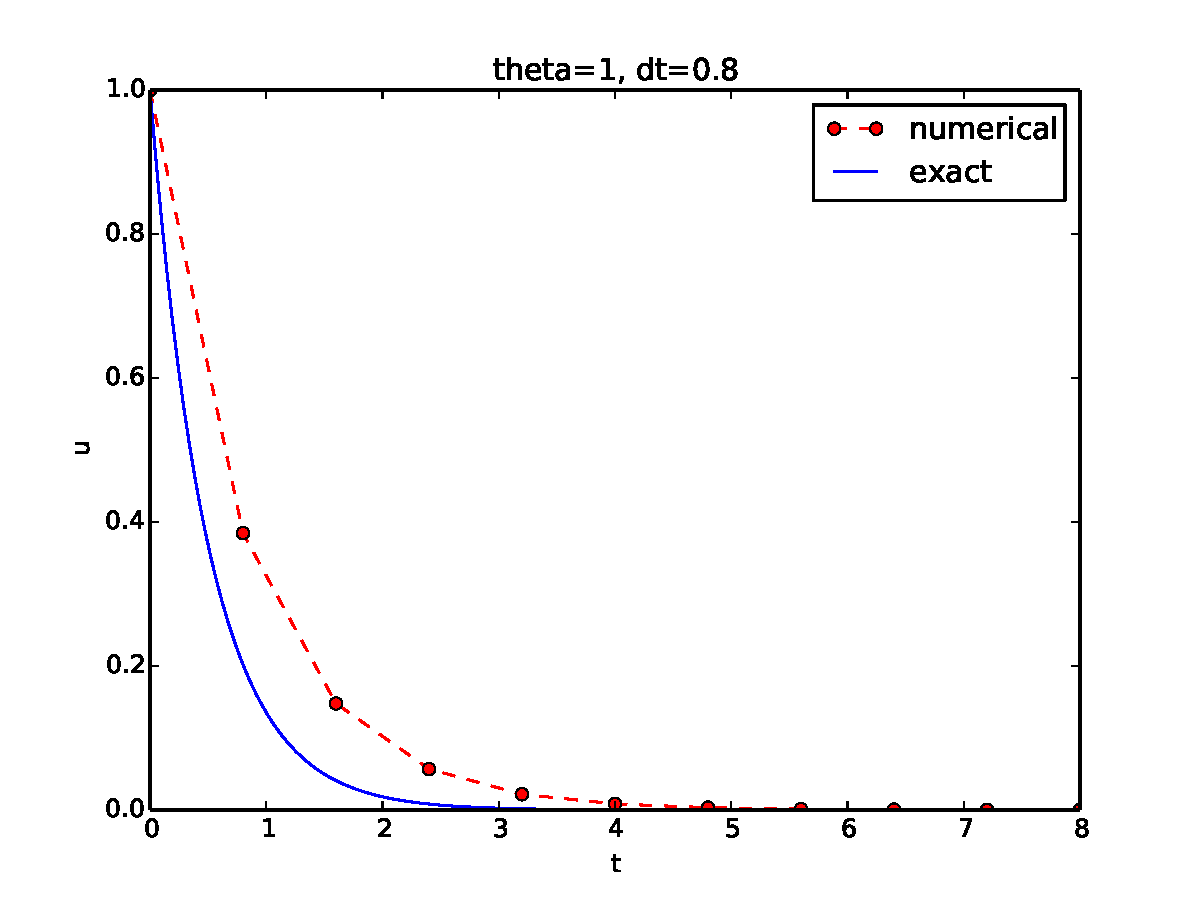
\includegraphics[width=0.8\linewidth]{fig-alg/decay_v2.pdf}}
  \caption{
  Comparison of numerical and exact solution. \label{decay:fig:v2}
  }
\end{figure}
%\clearpage % flush figures decay:fig:v2



\subsection{Verifying the implementation}

It is easy to make mistakes while deriving and implementing numerical
algorithms, so we should never believe in the solution before it has
been thoroughly verified.


\begin{notice_mdfboxadmon}[Verification and validation.]
The purpose of \emph{verifying} a program is to bring evidence for the
property that there are no errors in the implementation. A related
term, \emph{validate} (and \emph{validation}),
addresses the question if the ODE model is a good
representation of the phenomena we want to simulate. To remember the
difference between verification and validation, verification is
about \emph{solving the equations right}, while validation is about \emph{solving
the right equations}. We must always perform a verification before
it is meaningful to believe in the computations and perform validation
(which compares the program results with physical experiments or observations).
\end{notice_mdfboxadmon}




The most obvious idea for verification
in our case is to compare the numerical solution with the exact
solution, when that exists. This is, however, not a particularly good
method. The reason is that there will always
be a discrepancy
between these two solutions, due to numerical
approximations, and we cannot precisely quantify the approximation
errors. The open question is therefore whether we have the
mathematically correct
discrepancy or if we have another, maybe small,
discrepancy due to both an approximation error \emph{and} an error in the
implementation. It is thus
impossible to judge whether the program is correct or not by
just looking at the graphs in Figure~\ref{decay:fig:v2}.

To avoid
mixing the unavoidable numerical approximation errors and the
undesired implementation errors, we should try to make tests where
we have some exact
computation of the discrete solution or at least parts of it.
Examples will show how this can be done.

\paragraph{Running a few algorithmic steps by hand.}
The simplest approach to produce a correct non-trivial reference
solution for the discrete solution $u$, is to compute a few steps of
the algorithm by hand. Then we can compare the hand calculations with
numbers produced by the program.

A straightforward approach is to use a calculator and
compute $u^1$, $u^2$, and $u^3$. With $I=0.1$, $\theta=0.8$,
and $\Delta t =0.8$ we get

\[ A\equiv \frac{1 - (1-\theta) a\Delta t}{1 + \theta a \Delta t} = 0.298245614035\]
\begin{align*}
u^1 &= AI=0.0298245614035,\\ 
u^2 &= Au^1= 0.00889504462912,\\ 
u^3 &=Au^2= 0.00265290804728
\end{align*}

Comparison of these manual calculations with the result of the
\texttt{solver} function is carried out in the function

\begin{cod}{cbg_blue1}\begin{Verbatim}[numbers=none,fontsize=\fontsize{9pt}{9pt},baselinestretch=0.95,xleftmargin=2mm]
def test_solver_three_steps():
    """Compare three steps with known manual computations."""
    theta = 0.8; a = 2; I = 0.1; dt = 0.8
    u_by_hand = array([I,
                       0.0298245614035,
                       0.00889504462912,
                       0.00265290804728])

    Nt = 3  # number of time steps
    u, t = solver(I=I, a=a, T=Nt*dt, dt=dt, theta=theta)

    tol = 1E-15  # tolerance for comparing floats
    diff = abs(u - u_by_hand).max()
    success = diff <= tol
    assert success
\end{Verbatim}
\end{cod}
\noindent
The \Verb!test_solver_three_steps! function follows widely used conventions
for \emph{unit testing}. By following such conventions we can at a later
stage easily execute a big test suite for our software. That is, after
a small modification is made to the program, we can by typing just
a short command, run through a large number of tests to check that the
modifications do not break any computations.
The conventions boil down to three rules:

\begin{itemize}
 \item The test function name must start with \Verb!test_! and the function
   cannot take any arguments.

 \item The test must end up in a boolean expression that is \texttt{True} if
   the test was passed and \texttt{False} if it failed.

 \item The function must run \texttt{assert} on the boolean expression, resulting
   in program abortion (due to an \texttt{AssertionError} exception) if
   the test failed.
\end{itemize}

\noindent
The main program can routinely run the verification test prior to
solving the real problem:

\begin{cod}{cbg_blue1}\begin{Verbatim}[numbers=none,fontsize=\fontsize{9pt}{9pt},baselinestretch=0.95,xleftmargin=2mm]
test_solver_three_steps()
plot_numerical_and_exact(I=1, a=2, T=8, dt=0.8, theta=1)
show()
\end{Verbatim}
\end{cod}
\noindent
(Rather than calling \Verb!test_*()! functions explicitly, one will
normally ask a testing framework like nose
or pytest to find and run such functions.)
The complete program including the verification above is
found in the file \href{{http://tinyurl.com/ofkw6kc/alg/decay_v3.py}}{\nolinkurl{decay_v3.py}}.


\subsection{Computing the numerical error as a mesh function}
\label{decay:computing:error}

Now that we have some evidence for a correct implementation, we are in
position to compare the computed $u^n$ values in the \texttt{u} array with
the exact $u$ values at the mesh points, in order to study the error
in the numerical solution.

\index{representative (mesh function)}

A natural way to compare the exact and discrete solutions is to
calculate their difference as a mesh function for the error:

\begin{equation}
e^n = \uex(t_n) - u^n,\quad n=0,1,\ldots,N_t \tp
\end{equation}
We may view the mesh function
$\uex^n = \uex(t_n)$ as a representation of the continuous function $\uex(t)$
defined for all $t\in [0,T]$. In fact,
$\uex^n$ is often called the \emph{representative} of
$\uex$ on the mesh. Then, $e^n = \uex^n - u^n$ is clearly
the difference of two mesh functions.

The error mesh function $e^n$ can be computed by

\begin{cod}{cbg_blue1}\begin{Verbatim}[numbers=none,fontsize=\fontsize{9pt}{9pt},baselinestretch=0.95,xleftmargin=2mm]
u, t = solver(I, a, T, dt, theta)  # Numerical sol.
u_e = u_exact(t, I, a)             # Representative of exact sol.
e = u_e - u
\end{Verbatim}
\end{cod}
\noindent
Note that the mesh functions \texttt{u} and \Verb!u_e! are represented by arrays
and associated with the points in the array \texttt{t}.

\index{array arithmetics} \index{array computing} \index{vectorization}


\begin{notice_mdfboxadmon}[Array arithmetics.]
The last statements

\begin{cod}{cbg_blue1}\begin{Verbatim}[numbers=none,fontsize=\fontsize{9pt}{9pt},baselinestretch=0.95,xleftmargin=2mm]
u_e = u_exact(t, I, a)
e = u_e - u
\end{Verbatim}
\end{cod}
\noindent
demonstrate some standard examples of array arithmetics: \texttt{t} is an
array of mesh points that we pass to \Verb!u_exact!. This function
evaluates \texttt{-a*t}, which is a scalar times an array, meaning that
the scalar is multiplied with each array element.
The result is an array, let us call it \texttt{tmp1}. Then
\texttt{exp(tmp1)} means applying the exponential function to each element in
\texttt{tmp1}, giving an array, say \texttt{tmp2}. Finally, \texttt{I*tmp2} is computed
(scalar times array) and \Verb!u_e! refers to this array returned from
\Verb!u_exact!. The expression \Verb!u_e - u! is the difference between
two arrays, resulting in a new array referred to by \texttt{e}.

Replacement of array element computations inside a loop by array
arithmetics is known as \emph{vectorization}.
\end{notice_mdfboxadmon}



\subsection{Computing the norm of the error mesh function}
\label{decay:computing:error:norm}

\index{continuous function norms}
\index{norm!continuous}

Instead of working with the error $e^n$ on the entire mesh, we
often want a single number expressing the size of the error.
This is obtained by taking the norm of the error function.

Let us first define norms of a function $f(t)$
defined for all $t\in [0,T]$.
Three common norms are

\begin{align}
||f||_{L^2} &= \left( \int_0^T f(t)^2 dt\right)^{1/2},
\label{decay:norms:L2}\\ 
||f||_{L^1} &= \int_0^T |f(t)| dt,
\label{decay:norms:L1}\\ 
||f||_{L^\infty} &= \max_{t\in [0,T]}|f(t)|\tp
\label{decay:norms:Linf}
\end{align}
The $L^2$ norm (\ref{decay:norms:L2}) (``L-two norm'')
has nice mathematical properties and
is the most popular norm. It is a generalization
of the well-known Eucledian norm of vectors to functions.
The $L^1$ norm looks simpler and more intuitive, but has less
nice mathematical properties compared to the two other norms, so
it is much less used in computations.
The $L^\infty$ is also called the max norm or the supremum norm
and is widely used. It focuses on a single point with the largest
value of $|f|$, while the other norms measure average behavior of
the function.

In fact, there is a whole family of norms,

\begin{equation}
||f||_{L^p} = \left(\int_0^T f(t)^pdt\right)^{1/p},
\end{equation}
with $p$ real. In particular,
$p=1$ corresponds to the $L^1$ norm above while $p=\infty$ is the
$L^\infty$ norm.

\index{discrete function norms}
\index{mesh function norms}
\index{norm!discrete (mesh function)}

Numerical computations involving mesh functions need corresponding norms.
Given a set of function values, $f^n$, and some associated mesh points, $t_n$,
a numerical integration rule can be used to calculate the $L^2$ and
$L^1$ norms defined above. Imagining that the mesh function is extended
to vary linearly between the mesh points, the Trapezoidal rule is
in fact an exact integration rule. A possible modification of the $L^2$
norm for a mesh function $f^n$ on a uniform mesh with spacing $\Delta t$
is therefore the well-known Trapezoidal integration formula

\[ ||f^n|| = \left(\Delta t\left(\half(f^0)^2 + \half(f^{N_t})^2
+ \sum_{n=1}^{N_t-1} (f^n)^2\right)\right)^{1/2} \]
A common approximation of this expression, motivated by the
convenience of having a simpler formula, is

\[ ||f^n||_{\ell^2} = \left(\Delta t\sum_{n=0}^{N_t} (f^n)^2\right)^{1/2} \tp\]
This is called the discrete $L^2$ norm and denoted by $\ell^2$.
If $||f||_{\ell^2}^2$ (i.e., the square of the norm) is used
instead of the Trapezoidal integration formula,
the error
is $\Delta t((f^0)^2 + (f^{N_t})^2)/2$. This means that the
weights at the end points of the mesh function are perturbed,
but as $\Delta t\rightarrow 0$, the error from this perturbation goes
to zero. As long as we are consistent and
stick to one kind of integration
rule for the norm of a mesh function, the details and accuracy of this
rule is of no concern.

The three discrete norms for a mesh function $f^n$, corresponding to
the $L^2$, $L^1$, and $L^\infty$ norms of $f(t)$ defined above, are
defined by

\begin{align}
||f^n||_{\ell^2} &= \left( \Delta t\sum_{n=0}^{N_t} (f^n)^2\right)^{1/2},
\label{decay:norms:l2}\\ 
||f^n||_{\ell^1} &= \Delta t\sum_{n=0}^{N_t} |f^n|,
\label{decay:norms:l1}\\ 
||f^n||_{\ell^\infty} &= \max_{0\leq n\leq N_t}|f^n|\tp
\label{decay:norms:linf}
\end{align}

Note that the $L^2$, $L^1$, $\ell^2$, and $\ell^1$ norms depend on the
length of the interval of interest (think of $f=1$, then the
norms are proportional to $\sqrt{T}$ or $T$). In some applications it
is convenient to think of a mesh function as just a vector of function
values without any relation to the interval $[0,T]$.
Then one can replace $\Delta t$ by $T/N_t$ and simply drop $T$ (which
is just a common scaling factor in the norm,
independent of the vector of function
values). Moreover, people prefer
to divide by the total length of the vector, $N_t+1$, instead of $N_t$.
This reasoning gives rise to the \emph{vector norms} for a vector
$f=(f_0,\ldots,f_{N})$:

\begin{align}
||f||_2 &= \left( \frac{1}{N+1}\sum_{n=0}^{N} (f_n)^2\right)^{1/2},
\label{decay:norms:vl2}\\ 
||f||_1 &= \frac{1}{N+1}\sum_{n=0}^{N} |f_n|,
\label{decay:norms:vl1}\\ 
||f||_{\ell^\infty} &= \max_{0\leq n\leq N}|f_n|\tp
\label{decay:norms:vlinf}
\end{align}
Here we have used the common vector component notation with subscripts
($f_n$) and $N$ as length. We will mostly work with mesh functions
and use the discrete $\ell^2$
norm (\ref{decay:norms:l2}) or the max norm $\ell^\infty$
(\ref{decay:norms:linf}), but the corresponding vector norms
(\ref{decay:norms:vl2})-(\ref{decay:norms:vlinf}) are also much used
in numerical computations, so it is important to know the different
norms and the relations between them.

\index{error!norms}

A single number that expresses the size of the numerical error
will be taken as $||e^n||_{\ell^2}$ and called $E$:

\begin{equation}
E = \sqrt{\Delta t\sum_{n=0}^{N_t} (e^n)^2}
\label{decay:E}
\end{equation}
The corresponding Python code, using array arithmetics, reads

\begin{cod}{cbg_blue1}\begin{Verbatim}[numbers=none,fontsize=\fontsize{9pt}{9pt},baselinestretch=0.95,xleftmargin=2mm]
E = sqrt(dt*sum(e**2))
\end{Verbatim}
\end{cod}
\noindent
The \texttt{sum} function comes from \texttt{numpy} and computes the sum of the elements
of an array. Also the \texttt{sqrt} function is from \texttt{numpy} and computes the
square root of each element in the array argument.

\index{scalar computing}

\paragraph{Scalar computing.}
Instead of doing array computing \texttt{sqrt(dt*sum(e**2))} we can compute with
one element at a time:
\begin{cod}{cbg_blue1}\begin{Verbatim}[numbers=none,fontsize=\fontsize{9pt}{9pt},baselinestretch=0.95,xleftmargin=2mm]
m = len(u)     # length of u array (alt: u.size)
u_e = zeros(m)
t = 0
for i in range(m):
    u_e[i] = u_exact(t, a, I)
    t = t + dt
e = zeros(m)
for i in range(m):
    e[i] = u_e[i] - u[i]
s = 0  # summation variable
for i in range(m):
    s = s + e[i]**2
error = sqrt(dt*s)
\end{Verbatim}
\end{cod}
\noindent
Such element-wise computing, often called \emph{scalar} computing, takes
more code, is less readable, and runs much slower than what we
can achieve with array computing.





\subsection{Experiments with computing and plotting}


Let us write down a new function that wraps up the computation and all
the plotting statements used for comparing the exact and numerical
solutions. This function can be called with various $\theta$ and
$\Delta t$ values to see how the error depends on the method and mesh
resolution.

\begin{cod}{cbg_blue1}\begin{Verbatim}[numbers=none,fontsize=\fontsize{9pt}{9pt},baselinestretch=0.95,xleftmargin=2mm]
def explore(I, a, T, dt, theta=0.5, makeplot=True):
    """
    Run a case with the solver, compute error measure,
    and plot the numerical and exact solutions (if makeplot=True).
    """
    u, t = solver(I, a, T, dt, theta)    # Numerical solution
    u_e = u_exact(t, I, a)
    e = u_e - u
    E = sqrt(dt*sum(e**2))
    if makeplot:
        figure()                         # create new plot
        t_e = linspace(0, T, 1001)       # fine mesh for u_e
        u_e = u_exact(t_e, I, a)
        plot(t,   u,   'r--o')           # red dashes w/circles
        plot(t_e, u_e, 'b-')             # blue line for exact sol.
        legend(['numerical', 'exact'])
        xlabel('t')
        ylabel('u')
        title('theta=%g, dt=%g' % (theta, dt))
        theta2name = {0: 'FE', 1: 'BE', 0.5: 'CN'}
        savefig('%s_%g.png' % (theta2name[theta], dt))
        savefig('%s_%g.pdf' % (theta2name[theta], dt))
        show()
    return E
\end{Verbatim}
\end{cod}
\noindent

The \texttt{figure()} call is key: without it, a new \texttt{plot} command will
draw the new pair of curves in the same plot window, while we want
the different pairs to appear in separate windows and files.
Calling \texttt{figure()} ensures this.

Instead of including the $\theta$ value in the filename to implicitly
inform about the applied method, the code utilizes a little Python
dictionary that maps each relevant $\theta$ value to a corresponding
acronym for the method name (FE, BE, or CN):

\begin{cod}{cbg_blue1}\begin{Verbatim}[numbers=none,fontsize=\fontsize{9pt}{9pt},baselinestretch=0.95,xleftmargin=2mm]
theta2name = {0: 'FE', 1: 'BE', 0.5: 'CN'}
savefig('%s_%g.png' % (theta2name[theta], dt))
\end{Verbatim}
\end{cod}
\noindent

\index{PNG plot} \index{PDF plot} \index{EPS plot}
\index{viewing graphics files}

The \texttt{explore} function stores the plot in two different image file formats:
PNG and PDF. The PNG format is suitable for
being included in HTML documents, while the PDF format provides
higher quality for {\LaTeX} (i.e., \textsc{pdf}{\LaTeX}) documents.
Frequently used viewers for these
image files on Unix systems are \texttt{gv} (comes with Ghostscript)
for the PDF format and
\texttt{display} (from the ImageMagick software suite) for PNG files:

\begin{Verbatim}[frame=lines,label=\fbox{{\tiny Terminal}},framesep=2.5mm,framerule=0.7pt,fontsize=\fontsize{9pt}{9pt}]
Terminal> gv BE_0.5.pdf
Terminal> display BE_0.5.png
\end{Verbatim}

A main program may run a loop over the three methods (given by
their corresponding $\theta$ values)
and call \texttt{explore} to compute errors and make plots:

\begin{cod}{cbg_blue1}\begin{Verbatim}[numbers=none,fontsize=\fontsize{9pt}{9pt},baselinestretch=0.95,xleftmargin=2mm]
def main(I, a, T, dt_values, theta_values=(0, 0.5, 1)):
    print 'theta   dt       error'  # Column headings in table
    for theta in theta_values:
        for dt in dt_values:
            E = explore(I, a, T, dt, theta, makeplot=True)
            print '%4.1f %6.2f: %12.3E' % (theta, dt, E)

main(I=1, a=2, T=5, dt_values=[0.4, 0.04])
\end{Verbatim}
\end{cod}
\noindent
The file \href{{http://tinyurl.com/ofkw6kc/alg/decay_plot_mpl.py}}{\nolinkurl{decay_plot_mpl.py}}
contains the complete code with the functions above.
Running this program results in

\begin{Verbatim}[frame=lines,label=\fbox{{\tiny Terminal}},framesep=2.5mm,framerule=0.7pt,fontsize=\fontsize{9pt}{9pt}]
Terminal> python decay_plot_mpl.py
theta   dt       error
 0.0   0.40:    2.105E-01
 0.0   0.04:    1.449E-02
 0.5   0.40:    3.362E-02
 0.5   0.04:    1.887E-04
 1.0   0.40:    1.030E-01
 1.0   0.04:    1.382E-02
\end{Verbatim}
We observe that reducing $\Delta t$ by a factor of 10 increases the
accuracy for all three methods. We also see that
the combination of $\theta=0.5$ and a small time step $\Delta t =0.04$
gives a much more accurate solution, and that $\theta=0$ and $\theta=1$
with $\Delta t = 0.4$ result in the least accurate solutions.

Figure~\ref{decay:fig:FE1} demonstrates that the numerical solution
produced by the Forward Euler method with
$\Delta t=0.4$ clearly lies below the exact curve, but that the
accuracy improves considerably by reducing the time step by a factor
of 10.


\begin{figure}[!ht]  % decay:fig:FE1
  \centerline{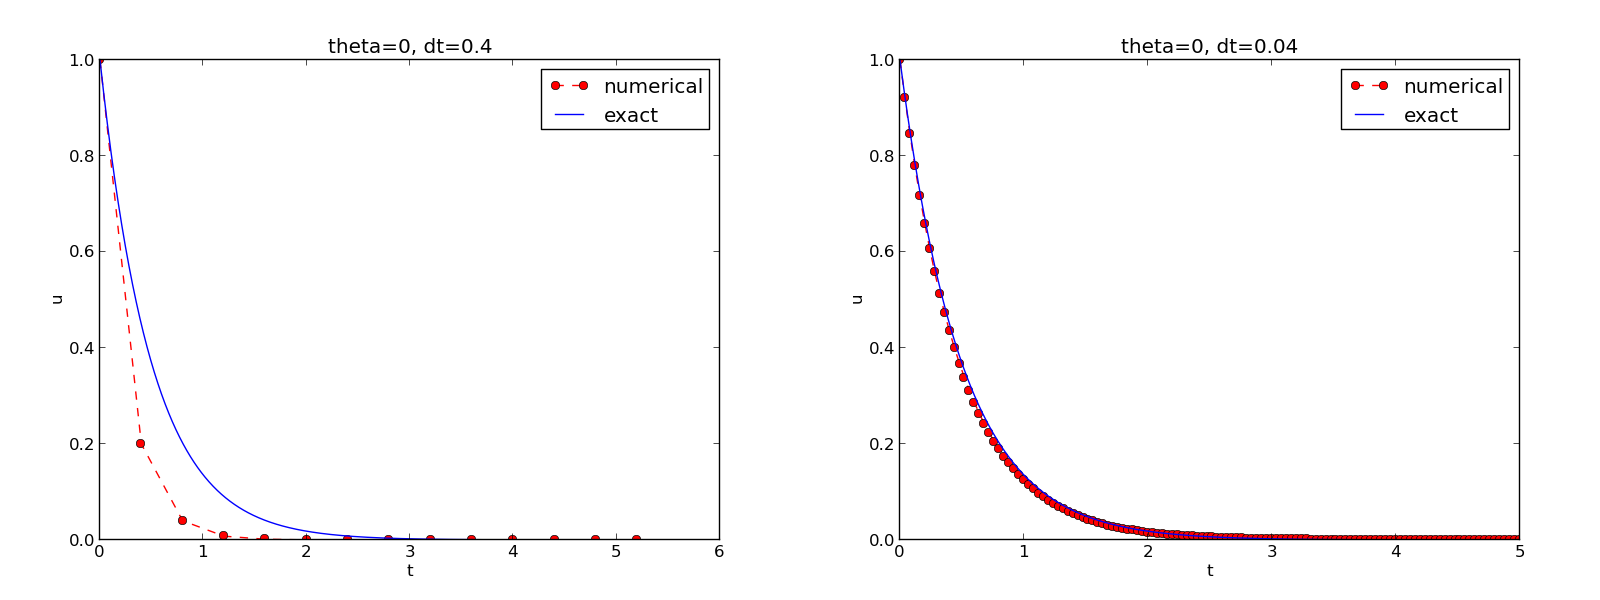
\includegraphics[width=1.1\linewidth]{fig-alg/FE1.png}}
  \caption{
  The Forward Euler scheme for two values of the time step. \label{decay:fig:FE1}
  }
\end{figure}
%\clearpage % flush figures decay:fig:FE1


The behavior of the two other schemes is shown in Figures~\ref{decay:fig:BE1}
and~\ref{decay:fig:CN1}. Crank-Nicolson is obviously the most accurate
scheme from this visual point of view.


\begin{figure}[!ht]  % decay:fig:BE1
  \centerline{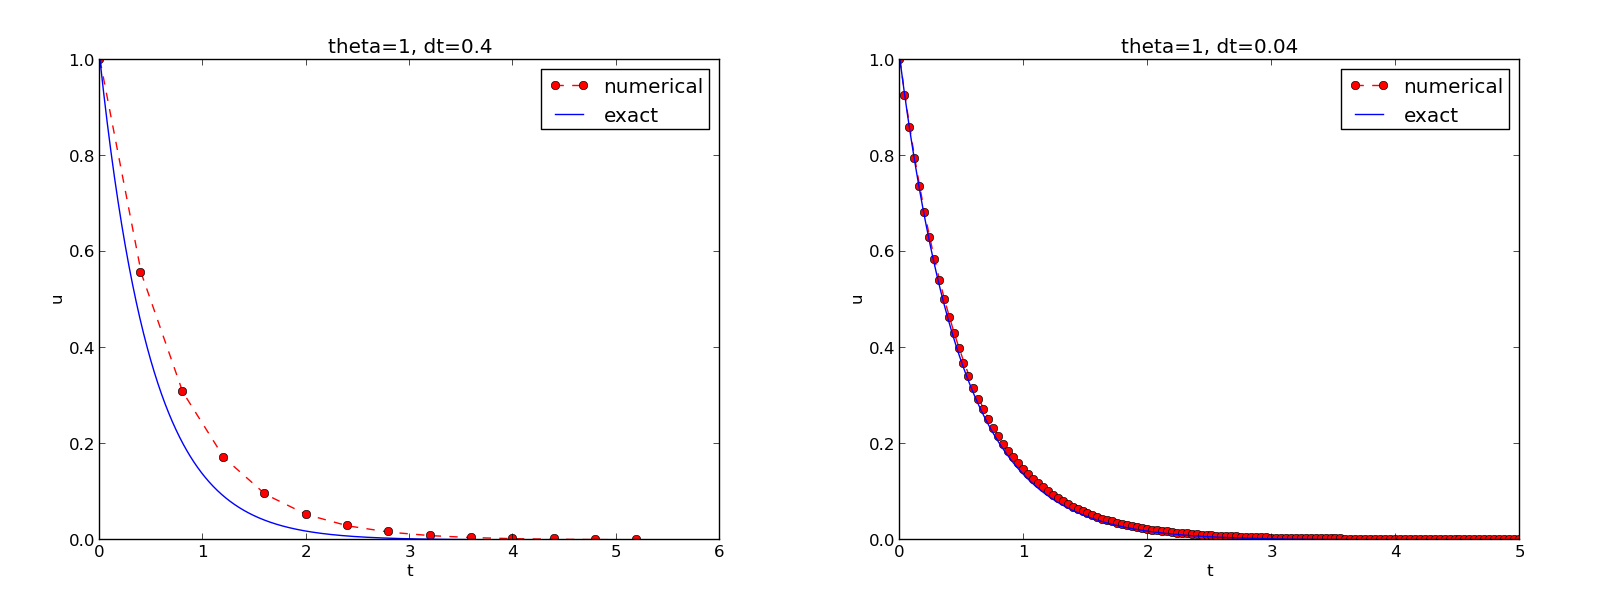
\includegraphics[width=1.1\linewidth]{fig-alg/BE1.png}}
  \caption{
  The Backward Euler scheme for two values of the time step. \label{decay:fig:BE1}
  }
\end{figure}
%\clearpage % flush figures decay:fig:BE1



\begin{figure}[!ht]  % decay:fig:CN1
  \centerline{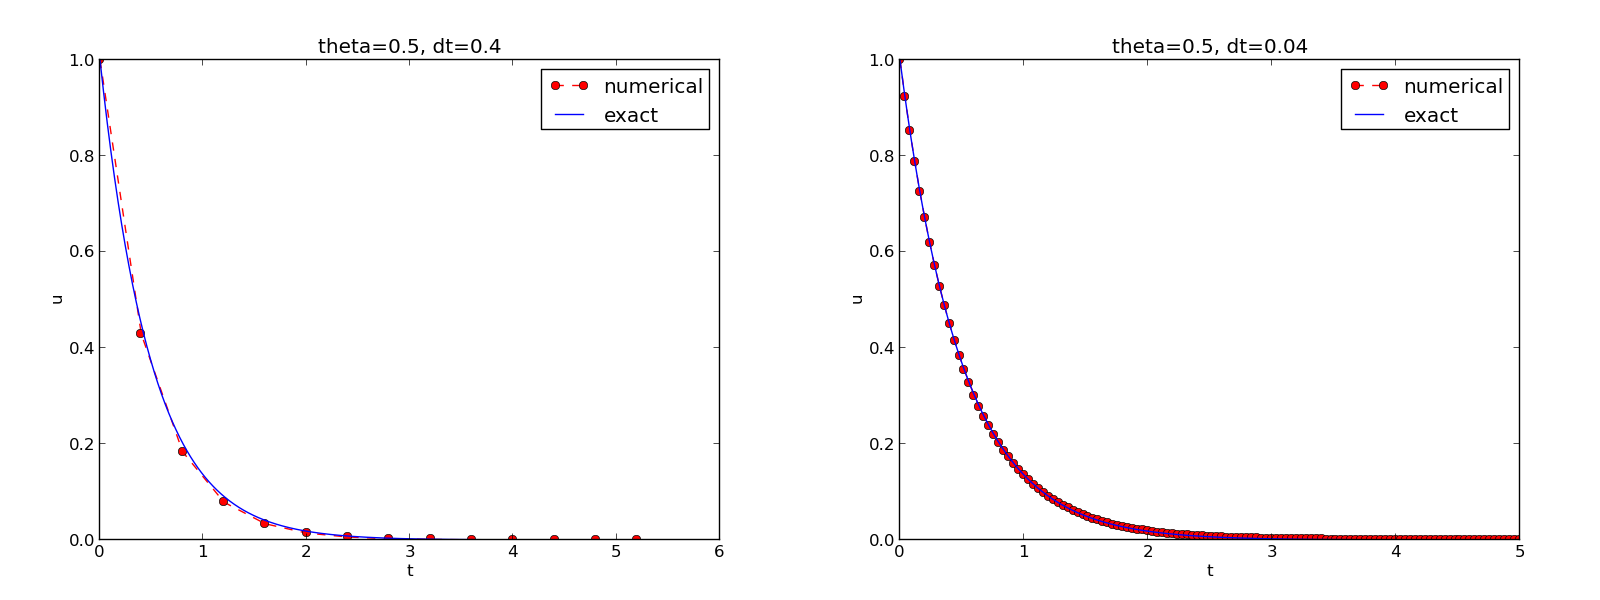
\includegraphics[width=1.1\linewidth]{fig-alg/CN1.png}}
  \caption{
  The Crank-Nicolson scheme for two values of the time step. \label{decay:fig:CN1}
  }
\end{figure}
%\clearpage % flush figures decay:fig:CN1



\index{cropping images}
\index{montage@{\rm\texttt{montage}} program}

\paragraph{Combining plot files.}
Mounting two PNG files beside each other, as done in Figures~\ref{decay:fig:FE1}-\ref{decay:fig:CN1}, is easily carried out by the
\href{{http://www.imagemagick.org/script/montage.php}}{\nolinkurl{montage}} program
from the ImageMagick suite:

\begin{Verbatim}[frame=lines,label=\fbox{{\tiny Terminal}},framesep=2.5mm,framerule=0.7pt,fontsize=\fontsize{9pt}{9pt}]
Terminal> montage -background white -geometry 100% -tile 2x1 \ 
          FE_0.4.png FE_0.04.png FE1.png
Terminal> convert -trim FE1.png FE1.png
\end{Verbatim}
The \texttt{-geometry} argument is used to specify the size of the image. Here,
we preserve the individual sizes of the images. The \texttt{-tile HxV} option
specifies \texttt{H} images in the horizontal direction and \texttt{V} images in
the vertical direction. A series of image files to be combined are then listed,
with the name of the resulting combined image, here \texttt{FE1.png} at the end.
The \texttt{convert -trim} command removes surrounding white areas in the figure
(an operation usually known as \emph{cropping} in image manipulation programs).

\index{pdftk@{\rm\texttt{pdftk}} program}
\index{pdfnup@{\rm\texttt{pdfnup}} program}
\index{pdfcrop@{\rm\texttt{pdfcrop}} program}

For {\LaTeX} reports it is not recommended to use \texttt{montage} and PNG files
as the result has too low resolution. Instead, plots should be made
in the PDF format and combined using the \texttt{pdftk}, \texttt{pdfnup}, and \texttt{pdfcrop} tools
(on Linux/Unix):

\begin{Verbatim}[frame=lines,label=\fbox{{\tiny Terminal}},framesep=2.5mm,framerule=0.7pt,fontsize=\fontsize{9pt}{9pt}]
Terminal> pdftk FE_0.4.png FE_0.04.png output tmp.pdf
Terminal> pdfnup --nup 2x1 --outfile tmp.pdf tmp.pdf
Terminal> pdfcrop tmp.pdf FE1.png  # output in FE1.png
\end{Verbatim}
Here, \texttt{pdftk} combines images into a multi-page PDF file, \texttt{pdfnup}
combines the images in individual pages to a table of images (pages),
and \texttt{pdfcrop} removes white margins in the resulting combined image file.


\paragraph{Plotting with SciTools.}
The \href{{https://github.com/hplgit/scitools}}{SciTools package} provides a
unified plotting interface, called Easyviz, to many different plotting
packages, including Matplotlib, Gnuplot, Grace, MATLAB,
VTK, OpenDX, and VisIt. The syntax is very similar to that of
Matplotlib and MATLAB. In fact, the plotting commands shown above look
the same in SciTool's Easyviz interface, apart from the import
statement, which reads

\begin{cod}{cbg_blue1}\begin{Verbatim}[numbers=none,fontsize=\fontsize{9pt}{9pt},baselinestretch=0.95,xleftmargin=2mm]
from scitools.std import *
\end{Verbatim}
\end{cod}
\noindent
This statement performs a \texttt{from numpy import *} as well as an import
of the most common pieces of the Easyviz (\texttt{scitools.easyviz}) package,
along with some additional numerical functionality.

With Easyviz one can
merge several plotting commands into a single one
using keyword arguments:

\begin{cod}{cbg_blue1}\begin{Verbatim}[numbers=none,fontsize=\fontsize{9pt}{9pt},baselinestretch=0.95,xleftmargin=2mm]
plot(t,   u,   'r--o',           # red dashes w/circles
     t_e, u_e, 'b-',             # blue line for exact sol.
     legend=['numerical', 'exact'],
     xlabel='t',
     ylabel='u',
     title='theta=%g, dt=%g' % (theta, dt),
     savefig='%s_%g.png' % (theta2name[theta], dt),
     show=True)
\end{Verbatim}
\end{cod}
\noindent
The \href{{http://tinyurl.com/ofkw6kc/alg/decay_plot_st.py}}{\nolinkurl{decay_plot_st.py}} file
contains such a demo.

By default, Easyviz employs Matplotlib for plotting, but \href{{http://www.gnuplot.info/}}{Gnuplot} and \href{{http://plasma-gate.weizmann.ac.il/Grace/}}{Grace} are viable alternatives:

\begin{Verbatim}[frame=lines,label=\fbox{{\tiny Terminal}},framesep=2.5mm,framerule=0.7pt,fontsize=\fontsize{9pt}{9pt}]
Terminal> python decay_plot_st.py --SCITOOLS_easyviz_backend gnuplot
Terminal> python decay_plot_st.py --SCITOOLS_easyviz_backend grace
\end{Verbatim}
The actual tool used for creating plots (called \emph{backend})
and numerous other options
can be permanently set in SciTool's configuration file.

All the Gnuplot windows are launched without any need to kill one before
the next one pops up (as is the case with Matplotlib) and one can
press the key 'q' anywhere in a plot window to kill it.
Another advantage of Gnuplot is the automatic choice of sensible
and distinguishable line types in black-and-white PDF and PostScript
files.

For more detailed information on syntax and plotting capabilities,
we refer to the Matplotlib \cite{Matplotlib:doc}
and SciTools \cite{SciTools:doc} documentation.
The hope is that
the programming syntax explained so far suffices for understanding the
basic plotting functionality and being able to look up
the cited technical documentation.




\subsection{Memory-saving implementation}

The computer memory requirements of our implementations so far consist
mainly of the \texttt{u} and \texttt{t} arrays, both of length $N_t+1$.  Also, for
the programs that involve array arithmetics, Python needs memory space
for storing temporary arrays. For example, computing \texttt{I*exp(-a*t)}
requires storing the intermediate result \texttt{a*t} before the preceding
minus sign can be applied. The resulting array is temporarily stored
and provided as input to the \texttt{exp} function.  Regardless of how we
implement simple ODE problems, storage requirements are very modest
and put no restrictions on how we choose our data structures and
algorithms.  Nevertheless, when the presented methods are applied to
three-dimensional PDE problems, memory storage requirements suddenly
become a challenging issue.

Let us briefly elaborate on how large the storage requirements can
quickly be in three-dimensional problems.  The PDE counterpart to our
model problem $u'=-a$ is a diffusion equation $u_t = a\nabla^2 u$
posed on a space-time domain. The discrete representation of this
domain may in 3D be a spatial mesh of $M^3$ points and a time mesh of
$N_t$ points.  In many applications, it is quite typical that $M$ is
at least 100, or even 1000.  Storing all the computed $u$ values, like
we have done in the programs so far, would demand storing arrays of
size up to $M^3N_t$. This would give a factor of $M^3$ larger storage
demands compared to what was required by our ODE programs. Each real
number in the \texttt{u} array requires 8 bytes (b) of storage. With $M=100$
and $N_t=1000$, there is a storage demand of $(10^3)^3\cdot 1000\cdot
8 = 8$ Gb for the solution array.  Fortunately, we can usually get rid
of the $N_t$ factor, resulting in 8 Mb of storage.  Below we explain
how this is done (the technique is almost always applied in
implementations of PDE problems).


Let us critically evaluate how much we really need to store in the
computer's memory for our implementation of the $\theta$ method. To
compute a new $u^{n+1}$, all we need is $u^n$. This implies that the
previous $u^{n-1},u^{n-2},\dots,u^0$ values do not need to be stored,
although this is convenient for plotting and data analysis in the
program.  Instead of the \texttt{u} array we can work with two variables for
real numbers, \texttt{u} and \Verb!u_1!, representing $u^{n+1}$ and $u^n$ in the
algorithm, respectively.  At each time level, we update \texttt{u} from \Verb!u_1!
and then set \Verb!u_1 = u!, so that the computed $u^{n+1}$ value becomes
the "previous" value $u^n$ at the next time level. The downside is
that we cannot plot the solution after the simulation is done since
only the last two numbers are available.  The remedy is to store
computed values in a file and use the file for visualizing the
solution later.

We have implemented this memory saving idea in the file
\href{{http://tinyurl.com/ofkw6kc/alg/decay_memsave.py}}{\nolinkurl{decay_memsave.py}}, which is a
slight modification of \href{{http://tinyurl.com/ofkw6kc/alg/decay_plot_mpl.py}}{\nolinkurl{decay_plot_mpl.py}} program.

The following function demonstrates how we work with the two most
recent values of the unknown:

\begin{cod}{cbg_blue1}\begin{Verbatim}[numbers=none,fontsize=\fontsize{9pt}{9pt},baselinestretch=0.95,xleftmargin=2mm]
def solver_memsave(I, a, T, dt, theta, filename='sol.dat'):
    """
    Solve u'=-a*u, u(0)=I, for t in (0,T] with steps of dt.
    Minimum use of memory. The solution is stored in a file
    (with name filename) for later plotting.
    """
    dt = float(dt)         # avoid integer division
    Nt = int(round(T/dt))  # no of intervals

    outfile = open(filename, 'w')
    # u: time level n+1, u_1: time level n
    t = 0
    u_1 = I
    outfile.write('%.16E  %.16E\n' % (t, u_1))
    for n in range(1, Nt+1):
        u = (1 - (1-theta)*a*dt)/(1 + theta*dt*a)*u_1
        u_1 = u
        t += dt
        outfile.write('%.16E  %.16E\n' % (t, u))
    outfile.close()
    return u, t
\end{Verbatim}
\end{cod}
\noindent
This code snippet also serves as a quick introduction to file writing in Python.
Reading the data in the file into arrays \texttt{t} and \texttt{u} is done by the
function

\begin{cod}{cbg_blue1}\begin{Verbatim}[numbers=none,fontsize=\fontsize{9pt}{9pt},baselinestretch=0.95,xleftmargin=2mm]
def read_file(filename='sol.dat'):
    infile = open(filename, 'r')
    u = [];  t = []
    for line in infile:
        words = line.split()
        if len(words) != 2:
            print 'Found more than two numbers on a line!', words
            sys.exit(1)  # abort
        t.append(float(words[0]))
        u.append(float(words[1]))
    return np.array(t), np.array(u)
\end{Verbatim}
\end{cod}
\noindent

This type of file with numbers in rows and columns is very common, and
\texttt{numpy} has a function \texttt{loadtxt} which loads such tabular data into a
two-dimensional array named by the user. Say the name is \texttt{data}, the
number in row \texttt{i} and column \texttt{j} is then \texttt{data[i,j]}.  The whole
column number \texttt{j} can be extracted by \texttt{data[:,j]}.  A version of
\Verb!read_file! using \texttt{np.loadtxt} reads

\begin{cod}{cbg_blue1}\begin{Verbatim}[numbers=none,fontsize=\fontsize{9pt}{9pt},baselinestretch=0.95,xleftmargin=2mm]
def read_file_numpy(filename='sol.dat'):
    data = np.loadtxt(filename)
    t = data[:,0]
    u = data[:,1]
    return t, u
\end{Verbatim}
\end{cod}
\noindent

The present counterpart to the \texttt{explore} function from
\href{{http://tinyurl.com/ofkw6kc/alg/decay_plot_mpl.py}}{\nolinkurl{decay_plot_mpl.py}} must run
\Verb!solver_memsave! and then load data from file before we can compute
the error measure and make the plot:

\begin{cod}{cbg_blue1}\begin{Verbatim}[numbers=none,fontsize=\fontsize{9pt}{9pt},baselinestretch=0.95,xleftmargin=2mm]
def explore(I, a, T, dt, theta=0.5, makeplot=True):
    filename = 'u.dat'
    u, t = solver_memsave(I, a, T, dt, theta, filename)

    t, u = read_file(filename)
    u_e = u_exact(t, I, a)
    e = u_e - u
    E = sqrt(dt*np.sum(e**2))
    if makeplot:
        figure()
        ...
\end{Verbatim}
\end{cod}
\noindent

Apart from the internal implementation, where $u^n$ values are stored
in a file rather than in an array, \Verb!decay_memsave.py! file works
exactly as the \Verb!decay_plot_mpl.py! file.

% !split
\section{Exercises}



% --- begin exercise ---
\begin{doconceexercise}
\refstepcounter{doconceexercisecounter}

\subsection*{Exercise \thedoconceexercisecounter: Define a mesh function and visualize it}

\label{decay:exer:meshfunc}


\subex{a)}
Write a function \Verb!mesh_function(f, t)! that returns an array with
mesh point values $f(t_0),\ldots,f(t_{N_t})$, where \texttt{f} is a Python
function implementing a mathematical function \texttt{f(t)} and $t_0,\ldots,t_{N_t}$
are mesh points stored in the array \texttt{t}. Use a loop over the mesh
points and compute one mesh function value at the time.


% removed !bsol ... !esol environment (because of the command-line option --without_solutions)

\subex{b)}
Use \Verb!mesh_function! to compute the mesh function corresponding to

\[
f(t) = \left\lbrace
\begin{array}{ll}
e^{-t},& 0\leq t\leq 3,\\ 
e^{-3t}, & 3 < t\leq 4
\end{array}\right.
\]
Choose a mesh $t_n=n\Delta t$ with $\Delta t=0.1$.
Plot the mesh function.


% removed !bsol ... !esol environment (because of the command-line option --without_solutions)



\noindent Filename: \Verb!mesh_function!.

% Closing remarks for this Exercise

\paragraph{Remarks.}
In Section~\ref{decay:computing:error} we show how easy it is to
compute a mesh function by array arithmetics (or array computing).
Using this technique, one could simply implement \Verb!mesh_function(f,t)!
as \texttt{return f(t)}. However, \texttt{f(t)} will not work if there are
if tests involving \texttt{t} inside \texttt{f} as is the case in b). Typically,
\texttt{if t < 3} must have \texttt{t < 3} as a boolean expression, but if \texttt{t} is
array, \texttt{t < 3}, is an \emph{array of boolean values}, which is not legal
as a boolean expression in an if test.
Computing one element
at a time as suggested in a) is a way of out of this problem.

We also remark that the function in b) is the solution of $u^{\prime}=-au$,
$u(0)=1$, for $t\in [0,4]$, where $a=1$ for $t\in [0,3]$ and $a=3$ for
$t\in [3,4]$.


\end{doconceexercise}
% --- end exercise ---




% --- begin exercise ---
\begin{doconceexercise}
\refstepcounter{doconceexercisecounter}

\subsection*{Problem \thedoconceexercisecounter: Differentiate a function}

\label{decay:exer:dudt}

\index{array arithmetics} \index{array computing} \index{vectorization}

Given a mesh function $u^n$ as an array \texttt{u} with $u^n$ values at mesh
points $t_n=n\Delta t$, the discrete derivative can be based on
centered differences:

\begin{equation}
d^n = [D_{2t}u]^n =
\frac{u^{n+1}-u^{n-1}}{2\Delta t},\quad n=1,\ldots,N_t-1\tp
\label{decay:exer:dudt:D2t}
\end{equation}
At the end points we use forward and backward differences:

\[ d^0 = [D_t^+u]^n = \frac{u^{1}-u^{0}}{\Delta t},\]
and

\[ d^{N_t} = [D_t^-u]^n = \frac{u^{N_t}-u^{N_t-1}}{\Delta t}\tp\]


\subex{a)}
Write a function
\texttt{differentiate(u, dt)} that returns the discrete derivative $d^n$ of the
mesh function $u^n$. The parameter \texttt{dt} reflects the
mesh spacing $\Delta t$. Write a corresponding test function
\Verb!test_differentiate()! for verifying the implementation.

% --- begin hint in exercise ---

\paragraph{Hint.}
The three differentiation formulas are
exact for quadratic polynomials. Use this property to verify the program.

% --- end hint in exercise ---


% removed !bsol ... !esol environment (because of the command-line option --without_solutions)

\subex{b)}
A standard implementation of the formula (\ref{decay:exer:dudt:D2t}) is to
have a loop over $i$. For large $N_t$, such loop may run slowly in
Python. A technique for speeding up the computations, called vectorization
or array computing,
replaces the loop by array operations. To see how this can be done in
the present mathematical problem, we
define two arrays

\begin{align*}
u^+ &= (u^2,u^3,\ldots,u^{N_t}),
u^- &= (u^0,u^1,\ldots,u^{N_t-2})\tp
\end{align*}
The formula (\ref{decay:exer:dudt:D2t}) can now be expressed as

\[ (d^1,d^2,\ldots,d^{N_t-1}) = \frac{1}{2\Delta t}(u^+ - u^-)\tp\]
The corresponding Python code reads

\begin{cod}{cbg_blue1}\begin{Verbatim}[numbers=none,fontsize=\fontsize{9pt}{9pt},baselinestretch=0.95,xleftmargin=2mm]
d[1:-1] = (u[2:] - u[0:-2])/(2*dt)
# or
d[1:N_t] = (u[2:N_t+1] - u[0:N_t-1])/(2*dt)
\end{Verbatim}
\end{cod}
\noindent
Recall that an array slice \texttt{u[1:-1]} contains the elements in \texttt{u} starting
with index 1 and going all indices up to, but not including, the last one
(\texttt{-1}).

Use the ideas above to implement a vectorized version of the
\texttt{differentiate} function without loops. Make a corresponding
test function that compares the result with that of
\texttt{differentiate}.


% removed !bsol ... !esol environment (because of the command-line option --without_solutions)

\noindent Filename: \texttt{differentiate}.

\end{doconceexercise}
% --- end exercise ---




% --- begin exercise ---
\begin{doconceexercise}
\refstepcounter{doconceexercisecounter}

\subsection*{Problem \thedoconceexercisecounter: Experiment with divisions}

\label{decay:exer:intdiv}

Explain what happens in the following computations, where
some are mathematically unexpected:

\begin{cod}{cbg_blue1}\begin{Verbatim}[numbers=none,fontsize=\fontsize{9pt}{9pt},baselinestretch=0.95,xleftmargin=2mm]
>>> dt = 3
>>> T = 8
>>> Nt = T/dt
>>> Nt
2
>>> theta = 1; a = 1
>>> (1 - (1-theta)*a*dt)/(1 + theta*dt*a)
0
\end{Verbatim}
\end{cod}
\noindent


% removed !bsol ... !esol environment (because of the command-line option --without_solutions)
\noindent Filename: \texttt{pyproblems}.

\end{doconceexercise}
% --- end exercise ---




% --- begin exercise ---
\begin{doconceexercise}
\refstepcounter{doconceexercisecounter}

\subsection*{Problem \thedoconceexercisecounter: Experiment with wrong computations}

\label{decay:exer:decay1err}

Consider the \texttt{solver} function in the \href{{http://tinyurl.com/ofkw6kc/alg/decay_v1.py}}{\nolinkurl{decay_v1.py}} file
and the following call:

\begin{cod}{cbg_blue1}\begin{Verbatim}[numbers=none,fontsize=\fontsize{9pt}{9pt},baselinestretch=0.95,xleftmargin=2mm]
u, t = solver(I=1, a=1, T=7, dt=2, theta=1)
\end{Verbatim}
\end{cod}
\noindent
The output becomes

\begin{cod}{cbg_blue1}\begin{Verbatim}[numbers=none,fontsize=\fontsize{9pt}{9pt},baselinestretch=0.95,xleftmargin=2mm]
t= 0.000 u=1
t= 2.000 u=0
t= 4.000 u=0
t= 6.000 u=0
\end{Verbatim}
\end{cod}
\noindent
Print out the result of all intermediate computations and use
\texttt{type(v)} to see the object type of the result stored in some variable \texttt{v}.
Examine the intermediate calculations and explain
why \texttt{u} is wrong and why we compute up to $t=6$ only even though we
specified $T=7$.


% removed !bsol ... !esol environment (because of the command-line option --without_solutions)
\noindent Filename: \Verb!decay_v1_err!.

\end{doconceexercise}
% --- end exercise ---




% --- begin exercise ---
\begin{doconceexercise}
\refstepcounter{doconceexercisecounter}

\subsection*{Problem \thedoconceexercisecounter: Plot the error function}

\label{decay:exer:plot:error}

Solve the problem $u'=-au$, $u(0)=I$, using the Forward Euler, Backward
Euler, and Crank-Nicolson schemes. For each scheme, plot the error mesh
function $e^n = \uex(t_n)-u^n$ for $\Delta t=0.1, 0.05, 0.025$,
where $\uex$ is the exact solution of the ODE and
$u^n$ is the numerical solution at mesh point $t_n$.

% --- begin hint in exercise ---

\paragraph{Hint.}
Modify the \href{{http://tinyurl.com/ofkw6kc/alg/decay_plot_mpl.py}}{\nolinkurl{decay_plot_mpl.py}} code.

% --- end hint in exercise ---


% removed !bsol ... !esol environment (because of the command-line option --without_solutions)
\noindent Filename: \Verb!decay_plot_error!.

\end{doconceexercise}
% --- end exercise ---




% --- begin exercise ---
\begin{doconceexercise}
\refstepcounter{doconceexercisecounter}

\subsection*{Problem \thedoconceexercisecounter: Change formatting of numbers and debug}

\label{decay:exer:inexact:output}

The \href{{http://tinyurl.com/ofkw6kc/alg/decay_memsave.py}}{\nolinkurl{decay_memsave.py}} program
writes the time values and solution values to a file which looks
like
\begin{cod}{cbg_blue1}\begin{Verbatim}[numbers=none,fontsize=\fontsize{9pt}{9pt},baselinestretch=0.95,xleftmargin=2mm]
0.0000000000000000E+00  1.0000000000000000E+00
2.0000000000000001E-01  8.3333333333333337E-01
4.0000000000000002E-01  6.9444444444444453E-01
6.0000000000000009E-01  5.7870370370370383E-01
8.0000000000000004E-01  4.8225308641975323E-01
1.0000000000000000E+00  4.0187757201646102E-01
1.2000000000000000E+00  3.3489797668038418E-01
1.3999999999999999E+00  2.7908164723365347E-01
\end{Verbatim}
\end{cod}
\noindent
Modify the file output such that it looks like
\begin{cod}{cbg_blue1}\begin{Verbatim}[numbers=none,fontsize=\fontsize{9pt}{9pt},baselinestretch=0.95,xleftmargin=2mm]
0.000  1.00000
0.200  0.83333
0.400  0.69444
0.600  0.57870
0.800  0.48225
1.000  0.40188
1.200  0.33490
1.400  0.27908
\end{Verbatim}
\end{cod}
\noindent
If you have just modified the formatting of numbers in the file,
running the modified program
\begin{Verbatim}[frame=lines,label=\fbox{{\tiny Terminal}},framesep=2.5mm,framerule=0.7pt,fontsize=\fontsize{9pt}{9pt}]
Terminal> python decay_memsave_v2.py --T 10 --theta 1 \ 
          --dt 0.2 --makeplot
\end{Verbatim}
leads to printing of the message \Verb?Bug in the implementation!? in the
terminal window. Why?


% removed !bsol ... !esol environment (because of the command-line option --without_solutions)
\noindent Filename: \Verb!decay_memsave_v2!.

\end{doconceexercise}
% --- end exercise ---


% !split


\bibliographystyle{plain}
\bibliography{../papers}

% ------------------- end of main content ---------------

% #ifdef PREAMBLE
\cleardoublepage\phantomsection  % trick to get correct link to Index
\printindex

\end{document}
% #endif

